\documentclass[
  stu,
  floatsintext,
  longtable,
  nolmodern,
  notxfonts,
  notimes,
  draftfirst,
  colorlinks=true,linkcolor=blue,citecolor=blue,urlcolor=blue]{apa7}

\usepackage{amsmath}
\usepackage{amssymb}




\RequirePackage{longtable}
\RequirePackage{threeparttablex}

\makeatletter
\renewcommand{\paragraph}{\@startsection{paragraph}{4}{\parindent}%
	{0\baselineskip \@plus 0.2ex \@minus 0.2ex}%
	{-.5em}%
	{\normalfont\normalsize\bfseries\typesectitle}}

\renewcommand{\subparagraph}[1]{\@startsection{subparagraph}{5}{0.5em}%
	{0\baselineskip \@plus 0.2ex \@minus 0.2ex}%
	{-\z@\relax}%
	{\normalfont\normalsize\bfseries\itshape\hspace{\parindent}{#1}\textit{\addperi}}{\relax}}
\makeatother




\usepackage{longtable, booktabs, multirow, multicol, colortbl, hhline, caption, array, float, xpatch}
\usepackage{subcaption}


\renewcommand\thesubfigure{\Alph{subfigure}}
\setcounter{topnumber}{2}
\setcounter{bottomnumber}{2}
\setcounter{totalnumber}{4}
\renewcommand{\topfraction}{0.85}
\renewcommand{\bottomfraction}{0.85}
\renewcommand{\textfraction}{0.15}
\renewcommand{\floatpagefraction}{0.7}

\usepackage{tcolorbox}
\tcbuselibrary{listings,theorems, breakable, skins}
\usepackage{fontawesome5}

\definecolor{quarto-callout-color}{HTML}{909090}
\definecolor{quarto-callout-note-color}{HTML}{0758E5}
\definecolor{quarto-callout-important-color}{HTML}{CC1914}
\definecolor{quarto-callout-warning-color}{HTML}{EB9113}
\definecolor{quarto-callout-tip-color}{HTML}{00A047}
\definecolor{quarto-callout-caution-color}{HTML}{FC5300}
\definecolor{quarto-callout-color-frame}{HTML}{ACACAC}
\definecolor{quarto-callout-note-color-frame}{HTML}{4582EC}
\definecolor{quarto-callout-important-color-frame}{HTML}{D9534F}
\definecolor{quarto-callout-warning-color-frame}{HTML}{F0AD4E}
\definecolor{quarto-callout-tip-color-frame}{HTML}{02B875}
\definecolor{quarto-callout-caution-color-frame}{HTML}{FD7E14}

%\newlength\Oldarrayrulewidth
%\newlength\Oldtabcolsep


\usepackage{hyperref}




\providecommand{\tightlist}{%
  \setlength{\itemsep}{0pt}\setlength{\parskip}{0pt}}
\usepackage{longtable,booktabs,array}
\usepackage{calc} % for calculating minipage widths
% Correct order of tables after \paragraph or \subparagraph
\usepackage{etoolbox}
\makeatletter
\patchcmd\longtable{\par}{\if@noskipsec\mbox{}\fi\par}{}{}
\makeatother
% Allow footnotes in longtable head/foot
\IfFileExists{footnotehyper.sty}{\usepackage{footnotehyper}}{\usepackage{footnote}}
\makesavenoteenv{longtable}

\usepackage{graphicx}
\makeatletter
\newsavebox\pandoc@box
\newcommand*\pandocbounded[1]{% scales image to fit in text height/width
  \sbox\pandoc@box{#1}%
  \Gscale@div\@tempa{\textheight}{\dimexpr\ht\pandoc@box+\dp\pandoc@box\relax}%
  \Gscale@div\@tempb{\linewidth}{\wd\pandoc@box}%
  \ifdim\@tempb\p@<\@tempa\p@\let\@tempa\@tempb\fi% select the smaller of both
  \ifdim\@tempa\p@<\p@\scalebox{\@tempa}{\usebox\pandoc@box}%
  \else\usebox{\pandoc@box}%
  \fi%
}
% Set default figure placement to htbp
\def\fps@figure{htbp}
\makeatother


% definitions for citeproc citations
\NewDocumentCommand\citeproctext{}{}
\NewDocumentCommand\citeproc{mm}{%
  \begingroup\def\citeproctext{#2}\cite{#1}\endgroup}
\makeatletter
 % allow citations to break across lines
 \let\@cite@ofmt\@firstofone
 % avoid brackets around text for \cite:
 \def\@biblabel#1{}
 \def\@cite#1#2{{#1\if@tempswa , #2\fi}}
\makeatother
\newlength{\cslhangindent}
\setlength{\cslhangindent}{1.5em}
\newlength{\csllabelwidth}
\setlength{\csllabelwidth}{3em}
\newenvironment{CSLReferences}[2] % #1 hanging-indent, #2 entry-spacing
 {\begin{list}{}{%
  \setlength{\itemindent}{0pt}
  \setlength{\leftmargin}{0pt}
  \setlength{\parsep}{0pt}
  % turn on hanging indent if param 1 is 1
  \ifodd #1
   \setlength{\leftmargin}{\cslhangindent}
   \setlength{\itemindent}{-1\cslhangindent}
  \fi
  % set entry spacing
  \setlength{\itemsep}{#2\baselineskip}}}
 {\end{list}}
\usepackage{calc}
\newcommand{\CSLBlock}[1]{\hfill\break\parbox[t]{\linewidth}{\strut\ignorespaces#1\strut}}
\newcommand{\CSLLeftMargin}[1]{\parbox[t]{\csllabelwidth}{\strut#1\strut}}
\newcommand{\CSLRightInline}[1]{\parbox[t]{\linewidth - \csllabelwidth}{\strut#1\strut}}
\newcommand{\CSLIndent}[1]{\hspace{\cslhangindent}#1}





\usepackage{newtx}

\defaultfontfeatures{Scale=MatchLowercase}
\defaultfontfeatures[\rmfamily]{Ligatures=TeX,Scale=1}





\title{Estimating the Unobserved: A Simulation Study on Censoring and
Truncation in Race Models of Choice and Response Time}


\shorttitle{Race Model Censoring and Truncation}


\usepackage{etoolbox}


\course{MI2324RM: Research Master's Internship}
\professor{Andrew Heathcote}
\duedate{May 25th, 2024}




\author{Jeroen E. Timmerman}



\affiliation{
{Department of Psychology, University of Amsterdam}}




\leftheader{Timmerman}



\abstract{This is my abstract. }

\keywords{censoring, truncation, missing data, evidence
accumulation, choice response data, diffusion decision model, linear
ballistic accumulator, Bayesian hierarchical modeling. decision making}

\authornote{\par{\addORCIDlink{Jeroen E.
Timmerman}{0009-0003-8208-0509}} 

\par{       }
\par{Correspondence concerning this article should be addressed
to Jeroen E. Timmerman, Department of Psychology, University of
Amsterdam, Nieuwe Achtergracht 129-B, Amsterdam, North-Holland 1018
WS, Email: \href{mailto:j.e.timmerman@uva.nl}{j.e.timmerman@uva.nl}}
}

\makeatletter
\let\endoldlt\endlongtable
\def\endlongtable{
\hline
\endoldlt
}
\makeatother

\urlstyle{same}



\makeatletter
\@ifpackageloaded{caption}{}{\usepackage{caption}}
\AtBeginDocument{%
\ifdefined\contentsname
  \renewcommand*\contentsname{Table of contents}
\else
  \newcommand\contentsname{Table of contents}
\fi
\ifdefined\listfigurename
  \renewcommand*\listfigurename{List of Figures}
\else
  \newcommand\listfigurename{List of Figures}
\fi
\ifdefined\listtablename
  \renewcommand*\listtablename{List of Tables}
\else
  \newcommand\listtablename{List of Tables}
\fi
\ifdefined\figurename
  \renewcommand*\figurename{Figure}
\else
  \newcommand\figurename{Figure}
\fi
\ifdefined\tablename
  \renewcommand*\tablename{Table}
\else
  \newcommand\tablename{Table}
\fi
}
\@ifpackageloaded{float}{}{\usepackage{float}}
\floatstyle{ruled}
\@ifundefined{c@chapter}{\newfloat{codelisting}{h}{lop}}{\newfloat{codelisting}{h}{lop}[chapter]}
\floatname{codelisting}{Listing}
\newcommand*\listoflistings{\listof{codelisting}{List of Listings}}
\makeatother
\makeatletter
\makeatother
\makeatletter
\@ifpackageloaded{caption}{}{\usepackage{caption}}
\@ifpackageloaded{subcaption}{}{\usepackage{subcaption}}
\makeatother

% From https://tex.stackexchange.com/a/645996/211326
%%% apa7 doesn't want to add appendix section titles in the toc
%%% let's make it do it
\makeatletter
\xpatchcmd{\appendix}
  {\par}
  {\addcontentsline{toc}{section}{\@currentlabelname}\par}
  {}{}
\makeatother

%% Disable longtable counter
%% https://tex.stackexchange.com/a/248395/211326

\usepackage{etoolbox}

\makeatletter
\patchcmd{\LT@caption}
  {\bgroup}
  {\bgroup\global\LTpatch@captiontrue}
  {}{}
\patchcmd{\longtable}
  {\par}
  {\par\global\LTpatch@captionfalse}
  {}{}
\apptocmd{\endlongtable}
  {\ifLTpatch@caption\else\addtocounter{table}{-1}\fi}
  {}{}
\newif\ifLTpatch@caption
\makeatother

\begin{document}

\maketitle


\setcounter{secnumdepth}{-\maxdimen} % remove section numbering

\setlength\LTleft{0pt}


\section{Introduction}\label{introduction}

Many paradigms in experimental psychology investigate speeded
decision-making, or are adapted to be speeded decision-making tasks.
There are two main outcome variables to these tasks: what choice someone
made (or whether this matches the corresponding stimulus), and how fast
someone made their choice. Researchers are often interested in the
conditions that affect these decisions and response times (RTs).

A problem arises when we want to make comparisons about the performance
on a task. Someone might be quicker to respond -- indicating better
performance, but at the same time they might be less accurate --
indicating worse performance. This is commonly referred to as the speed
accuracy trade-off, which complicates inferences on task performance.

A wide range of evidence accumulation models (EAMs) aim to model the
cognitive processes behind decision making as noisy accumulation of
evidence until a decision threshold is reached. This means that how fast
a participant is able to accumulate evidence towards a choice (the
evidence accumulation rate or drift rate) is modeled separately from a
participants' tendency to value speed over accuracy or vice versa (the
threshold). In addition to these decisional variables, EAMs often
estimate the non-decision time (the time it takes to encode the stimulus
and the time it takes to make the motor response for example), and they
often account for the variability within and between trials, as well as
response bias.

This paper will focus on three prominent EAMs that are supported by the
EMC2 package (\citeproc{ref-EMC2}{Stevenson et al., 2024}): the Linear
Ballistic Accumulator {[}LBA; Brown and Heathcote
(\citeproc{ref-LBA}{2008}){]}, the Racing Diffusion Model {[}RDM;
Tillman et al. (\citeproc{ref-RDM}{2020}){]}, and the Log-Normal Race
{[}LNR; Heathcote and Love (\citeproc{ref-LNR}{2012}){]}. These models
are race models, which model separate accumulators--or racers--for each
choice option, with the first racer to hit the threshold reflecting the
choice made. The time that it takes for the winning racer to hit the
threshold is the decision time, which makes up the RT together with the
non-decision time.

The LBA (\citeproc{ref-LBA}{Brown \& Heathcote, 2008}) models RTs and
responses as a race between deterministic linear accumulators, with the
slope for a racer drawn from \(\mathcal{N}(v, s_{v}^2)\), where \(v\) is
the mean evidence accumulation rate and \(s_v^2\) the between-trial
variance of the evidence accumulation rate. The intercept also has
between-trial variation and is drawn from \(\mathcal{U}(0,A)\), the
response threshold \(b = B + A\) (meaning that B is the distance from
the starting point variability to the response threshold), and the
non-decision time is \(t_0\). The line that intersects the threshold at
the lowest time determines the decision made, and the timepoint of the
intersection added to \(t_0\) is the RT (\citeproc{ref-LBA}{Brown \&
Heathcote, 2008}). The RDM (\citeproc{ref-RDM}{Tillman et al., 2020})
has a similar set of parameters, but instead of having between-trial
variation in evidence accumulation rate, the RDM has continuous normally
distributed variation within each trial. Lastly, the LNR is a race
between random samples from log-normal distributions, with the lowest
sample determining the choice and decision time, which is then added to
non-decision time \(t_0\) to constitute the RT. This means that the LNR
has three main parameters: the scale \(m\) of the lognormal, the shape
\(s\) of the lognormal, and the non-decision time \(t_0\)
(\citeproc{ref-LNR}{Heathcote \& Love, 2012}).
Figure~\ref{fig-racemodels} illustrates the dynamics of each model, with
A set to 0 for the RDM to reflect the parameters used in this paper.

\phantomsection\label{cell-fig-racemodels}
\begin{figure}[H]

{\caption{{Simple Race Model Illustrations}{\label{fig-racemodels}}}}

\pandocbounded{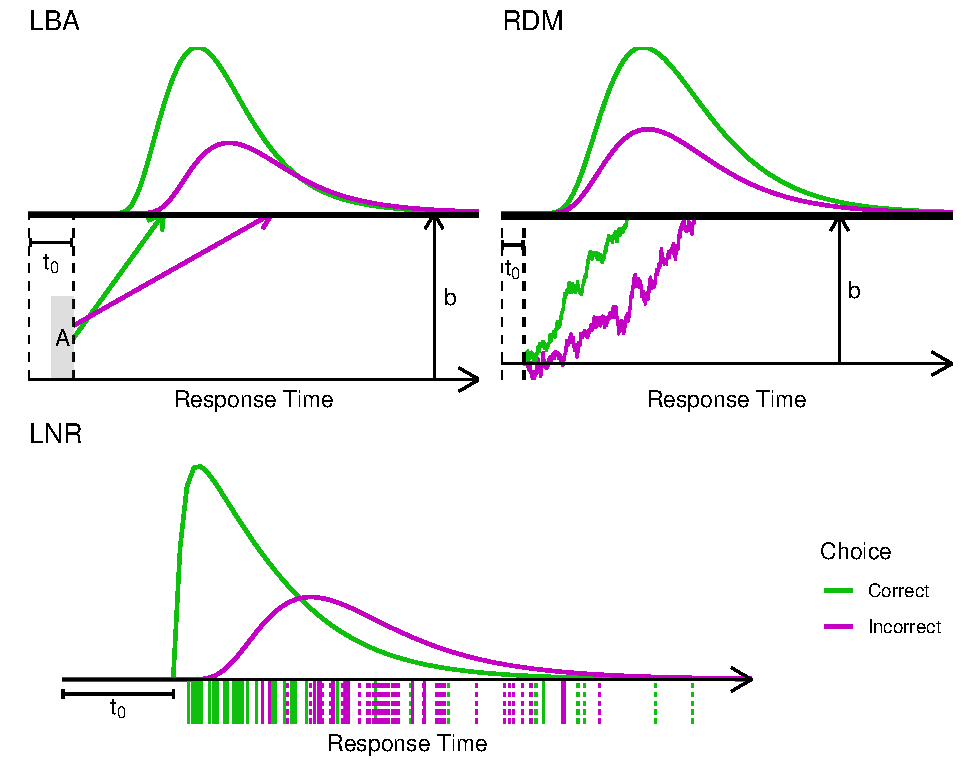
\includegraphics[keepaspectratio]{index_files/figure-pdf/fig-racemodels-1.pdf}}

{\noindent \emph{Note.} The dynamics of the race models in this paper
are illustrated here. The Linear Ballistic Accumulator (LBA) accumulates
evidence in a linear deterministic fashion, with normally distributed
variability \(s_v^2\) in slope \(v\) and uniformly distributed
variability \(A\) in starting point between trials. The Racing Diffusion
Model (RDM) has continuous normally distributed variance \(s_v^2\)
within the trial instead (diffusion), and can include starting point
variability between trials like the LBA, although this is not the case
for simulations in this paper. The Log-Normal Race (LNR) samples
accumulation times (vertical lines) from log-normal distributions, with
the shortest accumulation time (solid vertical lines) determining the
choice and the decision time.}

\end{figure}

Each of these race models have defined probability density functions
\(p(t \mid \boldsymbol{\theta})\) and cumulative density functions
\(P(t \mid \boldsymbol{\theta})\) for the finishing time of a single
accumulator. To compute the likelihood of parameter vector
\(\boldsymbol{\theta}\) for a trial, we can take the probability density
at that trial's RT for the parameter vector \(\boldsymbol{\theta}_i\)
corresponding to the choice \(i\), and multiply it by the probability of
the other accumulators \(j\) not finishing before accumulator \(i\):
\begin{equation}\phantomsection\label{eq-race-likelihood}{
\mathcal{L}(\boldsymbol{\theta} | t, i) = p(t \mid \boldsymbol{\theta}_{i}) \prod_{j \neq i}{1 - P(t \mid \boldsymbol{\theta}_{j})},
}\end{equation} which, as a function of \(t\), is the ``defective
distribution'' for \(i\), meaning that it integrates to the probability
of response \(i\).

Complicating the modelling of speeded decision making, RTs and choices
are often missing on certain trials due to experimental design. A
researcher may want to limit slow RTs in their experiment design, for
example to reduce slow type II thinking
(\citeproc{ref-dualprocess}{Evans, 2003}), or to emphasise speed.
Alternatively, researchers may want to remove outlying responses that
cannot have come from the process of interest (e.g., a response 0.05
seconds after stimulus onset, which is too fast for a decision making
process to occur).

There are two main ways to handle missing values: truncation, which
discards missing values with no assumption of the underlying
distribution, and censoring, which assumes the proportion of missing
values to reflect the true distribution, and takes this into account in
the model estimation.

Although truncation could potentially improve parameter estimates by
eliminating irrelevant outliers, outlier removal often increases
estimation bias by excluding extreme but valid RTs
(\citeproc{ref-MLcensoring}{Dolan et al., 2002};
\citeproc{ref-miller}{Miller, 2023};
\citeproc{ref-outliersRatcliff}{Ratcliff, 1993};
\citeproc{ref-ulrichmiller}{Ulrich \& Miller, 1994}). When truncation is
used for missing values due to response windows, this could even exclude
less extreme values, leading to more estimation bias.
Figure~\ref{fig-LBAtrunc} illustrates how upper truncation might distort
parameter estimation in a simple two forced choice decision task with
slow errors. Trials with slower accumulation rates--which tend to result
in more incorrect trials--get discarded, while trials with higher
accumulation rates are used to estimate the underlying parameters.

\phantomsection\label{cell-fig-LBAtrunc}
\begin{figure}[H]

{\caption{{Illustration of Missing Upper Response Times in the Linear
Ballistic Accumulator}{\label{fig-LBAtrunc}}}}

\pandocbounded{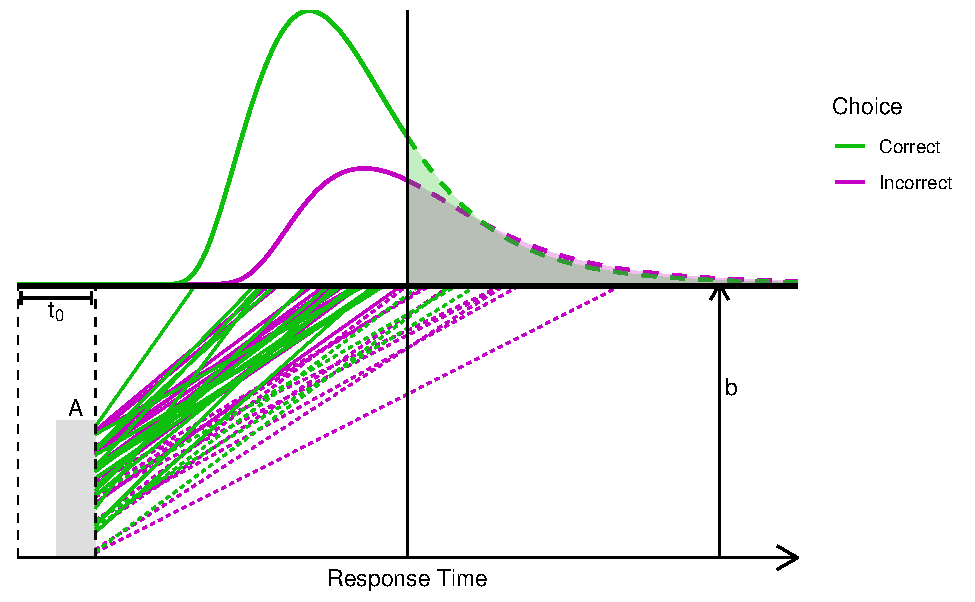
\includegraphics[keepaspectratio]{index_files/figure-pdf/fig-LBAtrunc-1.pdf}}

{\noindent \emph{Note.} This figure illustrates how upper censoring and
truncation relate to the LBA and the defective density. Dashed lines
represent the missing RT trials.}

\end{figure}

Despite the issues, many researchers still regularly implement
truncation, perhaps because of common practice, or because computing the
likelihood for a censored RT requires computing the area under the curve
of the likelihood function over the censored range, which can be slow to
compute. For race models, this means that we integrate
Equation~\ref{eq-race-likelihood} over the censored time range \(R\):
\begin{equation}\phantomsection\label{eq-censoring}{
\mathcal{L}(\boldsymbol{\theta} \mid t \in R, i) = \int_{R} p(t \mid \boldsymbol{\theta}_{i}) \prod_{j \neq i}{1 - P(t \mid \boldsymbol{\theta}_{j})} \, dt.
}\end{equation}

Equation~\ref{eq-censoring} can also be extended to accomodate missing
responses in addition to missing RTs by summing
Equation~\ref{eq-censoring} for each accumulator, resulting in the total
probability of any response in time range \(R\). Similarly, if we
censored both fast and slow responses with no distinction between the
two, we can sum the integrals over the lower and the upper range. We can
even combine censoring and truncation with
\begin{equation}\phantomsection\label{eq-censoringandtruncation}{
\mathcal{L}(\boldsymbol{\theta} \mid t \in R, i) \frac{\mathcal{L}(\boldsymbol{\theta} \mid 0 \leq t < \infty, i)}{\mathcal{L}(\boldsymbol{\theta} \mid t \in S, i)},
}\end{equation} where \(S\) is the range of all untruncated values.

Although censoring has been shown to result in more accurate parameter
recovery than truncation in common RT distributions
(\citeproc{ref-MLcensoring}{Dolan et al., 2002}), this has not yet been
established for race models. As data are routinely censored or
truncated, this study aims to compare parameter recovery for different
levels of censoring and truncation for the LBA, LNR, and RDM. We will
examine differences between the models in sensitivity to censoring and
truncation, and to what extent different levels of censoring and/or
truncation cause estimation bias and/or imprecision in designs with
varying numbers of trials.

Parameter estimates are expected to deteriorate fast with increased
truncation, while increased censoring is expected to result in smaller
and less biased deterioration of parameter recovery. Parameter posterior
distributions are expected to be overconfident for truncation, whereas
posterior distributions are expected to proportionally decrease in
confidence with increased censoring.

\section{Methods}\label{methods}

We compared RT censoring and truncation on parameter recovery in two
simulation studies. The first simulation study compared upper censoring
and truncation with responses known in a large number of samples to
assess asymptotic parameter identifiability. The second simulation study
assessed parameter recovery on a smaller number of trials to evaluate
the practical differences between censoring and truncation, comparing a
larger number of missing data scenarios.

To assess parameter identifiability, we first simulated data using known
parameters, which we then fit the same model to. This allows us to
compare the known, ``true'' parameter values with our fitted parameter
values. The code for all analyses and data generation are available on
https://github.com/timmerj1/censoring-truncation-study-EAMs.

For both simulation studies, a simple model with two stimuli and two
racers was used to generate the data. Conventional constants for the
LBA's (\(s_v = 1\)) and the RDM's drift rate variance (\(s = 1\)) were
used to generate and fit the data. Parameter values were chosen to
reflect common RT and choice distributions in simple two forced choice
tasks (see Table~\ref{tbl-pars} for an overview of parameters used). For
the LBA, decision thresholds were defined with \(B = b - A\). As is the
default in EMC2, parameters on the positive real line were log
transformed. Data was generated using the \texttt{make\_data} function
from EMC2 (\citeproc{ref-EMC2}{Stevenson et al., 2024}).

\begin{table}

{\caption{{Race Model Simulation Parameters}{\label{tbl-pars}}}}

\begin{tabular}[t]{llllll}
\toprule
\multicolumn{2}{c}{LBA} & \multicolumn{2}{c}{LNR} & \multicolumn{2}{c}{RDM} \\
\cmidrule(l{3pt}r{3pt}){1-2} \cmidrule(l{3pt}r{3pt}){3-4} \cmidrule(l{3pt}r{3pt}){5-6}
\multicolumn{1}{c}{Parameter} & \multicolumn{1}{c}{Value} & \multicolumn{1}{c}{Parameter} & \multicolumn{1}{c}{Value} & \multicolumn{1}{c}{Parameter} & \multicolumn{1}{c}{Value} \\
\cmidrule(l{3pt}r{3pt}){1-1} \cmidrule(l{3pt}r{3pt}){2-2} \cmidrule(l{3pt}r{3pt}){3-3} \cmidrule(l{3pt}r{3pt}){4-4} \cmidrule(l{3pt}r{3pt}){5-5} \cmidrule(l{3pt}r{3pt}){6-6}
$B$ & 2 & $m$ & 0.75 & $B$ & 3\\
$v$ & 3 & $m_{true}$ & 0.65 & $v$ & 1\\
$v_{true}$ & 1 & $s$ & 0.5 & $v_{true}$ & 4\\
$A$ & 2 & $s_{true}$ & 0.8 & $s_{true}$ & 0.75\\
$s_{v_{true}}$ & 0.75 & $t_0$ & 0.4 & $t_0$ & 0.2\\
\addlinespace
$B$ & 2 &  &  &  & \\
\bottomrule
\end{tabular}

{\noindent \emph{Note.} Parameters used to simulate response time and
choice data for study 1 and 2. Note that parameters on the real positive
line are estimated on a log scale in EMC2. Subscript `true' relates to a
match between stimulus and choice (a correct choice is made), and these
parameters are added to the corresponding parameter for the non-matching
racer.}

\end{table}

For the first simulation, upper censoring and truncation were compared
using a large number of trials (20,000 trials) to investigate the
differences between censoring and truncation without fits being affected
by random error. RTs were cut off at three different levels: at 2.5\%,
10\%, and 30\% of upper values, with cutoff points estimated in a
separate simulation of 20,000 trials. Responses were not missing for any
of the censored values. For each combination of model and missing level,
new data was simulated, but censoring and truncation were compared on
the same datasets to ensure differences cannot be caused by random
sampling error.

In the second simulation, a factorial design was used to vary whether
responses were known or unknown, which tail missed response times
(lower, upper, or both tails), the percentage of missing responses (2\%,
10\%, 30\%, or 50\%), and whether missing responses were censored or
truncated. For each condition, ten samples with a small number of trials
(400 trials) were simulated and fit. Missing level cutoffs were chosen
using the quantiles on a non-missing simulation with 4000 trials.

Parameter posteriors were sampled using the particle Metropolis within
Gibbs (PMwG) sampler in EMC2 (\citeproc{ref-EMC2}{Stevenson et al.,
2024}) using its default (standard normal) priors for non-hierarchical
estimation. Three PMwG chains were sampled for each parameter, with 50
particles per parameter (\citeproc{ref-PMwG}{\textbf{PMwG?}}).

To assess parameter recovery, we used the Root Mean Squared Errors
(RMSEs) between the posterior medians \(\boldsymbol{\hat{\theta}}\) and
the true parameters \(\boldsymbol{\theta}\):
\begin{equation}\phantomsection\label{eq-RMSE}{
RMSE = \sqrt{\frac{1}{n}\sum_{i=1}^{n}{(\hat{\theta}_i - \theta_i)^2}}.
}\end{equation}

Since we used Bayesian methods, the parameter estimates are not
restricted to point estimates. We will compute the quadratic Wasserstein
distance between the full posterior \(P\) samples \(X_1,...,X_n\) and
Dirac point mass distribution \(\delta_{\boldsymbol{\theta}}\) at the
true parameters \(\boldsymbol{\theta}\):
\begin{equation}\phantomsection\label{eq-Wasserstein}{
W_2(\delta_{\boldsymbol{\theta}}, P) = \sqrt{\frac{1}{n} \sum_{i=1}^{n}{\|X_i - \boldsymbol{\theta}\|^2}}.
}\end{equation} The Wasserstein distance was taken for the full model
using the Euclidean distance, as well as for the separate parameters
with unidimensional distance. The quadratic Wasserstein distance
simplifies to the RMSE if point estimates were used. Moreover, the
quadratic Wasserstein over a single dimension becomes an unbiased
estimate of the standard deviation when \(\theta\) is the mean of \(P\).
This makes the quadratic Wasserstein distance an interesting Bayesian
alternative to the RMSE.

For completeness, additional Pearson's correlation coefficients and mean
absolute errors were computed, but since these did not differ
substantially from the RMSE and \(W_2\), these statistics were plotted
in the appendix. All metrics in this paper and the appendix were
computed using the transformations of EMC2, meaning that parameters with
a ``natural zero'' point were log transformed to be estimated on the
entire real scale.

\section{Results}\label{results}

\section{Study 1: Upper Censoring}\label{study-1-upper-censoring}

Figure~\ref{fig-RMSE-upper} shows the RMSE between the true parameter
values and the medians of the posterior distribution for each fit. As
expected, both distance measures RMSE and \(W_2\) increase with an
increase of percentage missing for truncation. For censoring, the
distance measures stay closer to 0 and do not clearly increase when data
is censored rather than truncated. This indicates that censoring did
improve the parameter recovery in an asymptotic fit as expected. The
only case where censoring does not seem to outperform truncation is for
the RDM, where 2.5\% truncation did not perform worse than 2.5\%
censoring. With higher missing percentages, censoring still outperformed
truncation for the RDM.

\phantomsection\label{cell-fig-RMSE-upper}
\begin{figure}[H]

{\caption{{Root Mean Squared Errors and Quadratic Wasserstein Distances
for Upper Censoring}{\label{fig-RMSE-upper}}}}

\pandocbounded{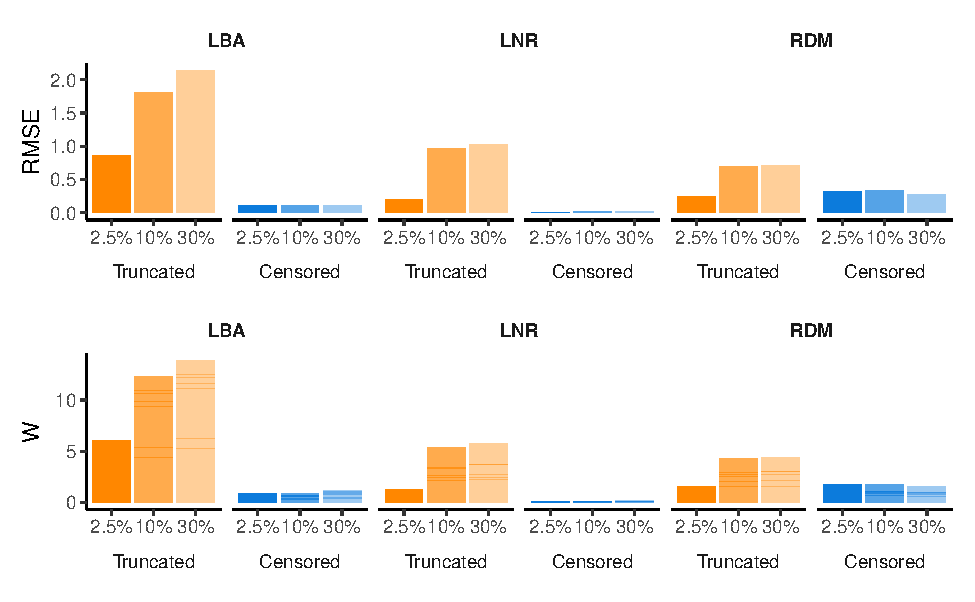
\includegraphics[keepaspectratio]{index_files/figure-pdf/fig-RMSE-upper-1.pdf}}

{\noindent \emph{Note.} For each model and each level of missingness,
the root mean squared errors (RMSE) and quadratic Wasserstein distances
(\(W_2\)) were computed and plotted. Lower RMSE and \(W_2\) indicate
better parameter recovery.}

\end{figure}

Looking at the credible intervals for each parameter in
Figure~\ref{fig-upper-censoring-recoveries}, the generally higher RMSE
for RDMs is explained by a general tendency for \(B\) and \(v\) to be
overestimated, while \(v_{win}\) and \(t_0\) are underestimated.
Overall, these parameters still seem to be recovered better with
censoring than with truncation, except that \(t_0\) and \(s_{win}\) were
recovered slightly better for truncation at a low percentage in this
simulation. For the other models, censoring clearly performs better than
truncation, with true parameters included by most credible intervals for
censoring, while most truncation credible intervals exclude the true
parameters. The main exception to this is the \(s_{win}\) parameter for
the LNR, where the credible interval for 30\% censoring does not include
the true parameter value.

\phantomsection\label{cell-fig-upper-censoring-recoveries}
\begin{figure}[H]

{\caption{{Parameter Recovery Plots for Upper Censoring /
Truncation}{\label{fig-upper-censoring-recoveries}}}}

\pandocbounded{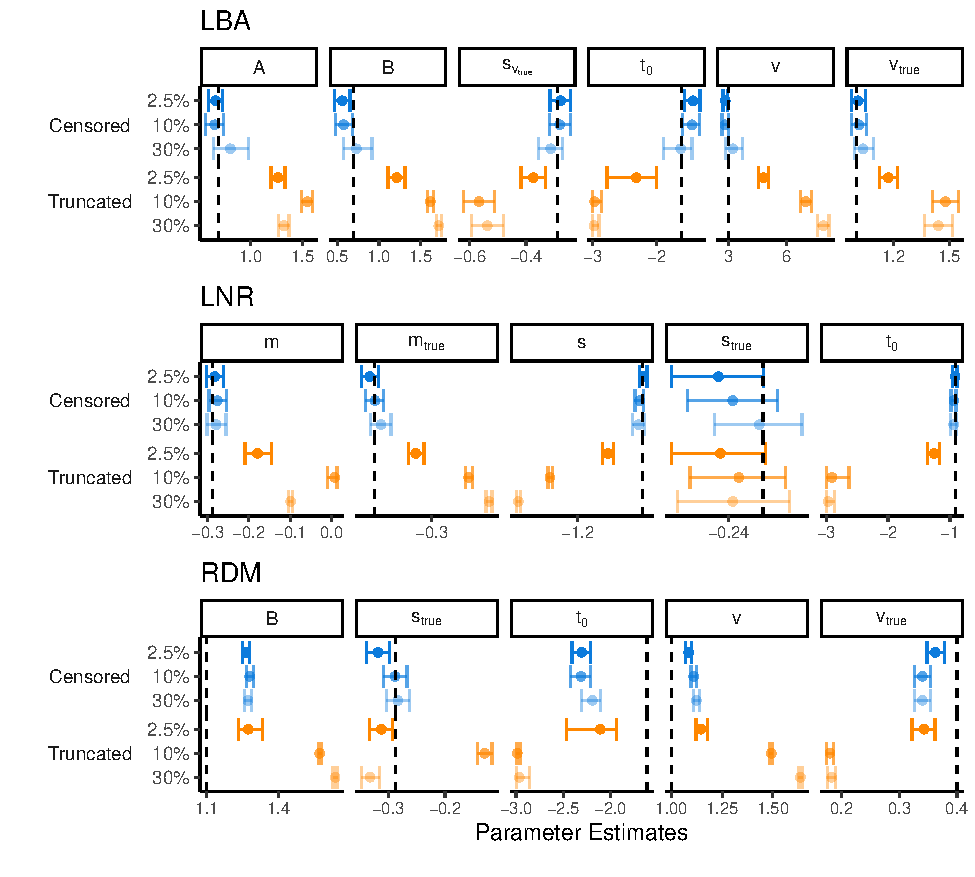
\includegraphics[keepaspectratio]{index_files/figure-pdf/fig-upper-censoring-recoveries-1.pdf}}

{\noindent \emph{Note.} Race model recoveries separated by model (LBA,
LNR and RDM) and censoring vs truncation. Especially the LBA and LNR
parameters are on the identity line for censoring, but off the line for
truncation.}

\end{figure}

Overall, these results indicate that upper censoring results in better
parameter recovery than upper truncation in an asymptotic sample,
i.e.~with a large number of trials. This cannot yet be generalized to
smaller sample sizes, as random error and parameter tradeoffs might
affect parameter recovery more than censoring versus truncation does.
Moreover, one might want to use lower censoring or truncation instead,
or a combination of lower and upper censoring or truncation. Lastly, in
this simulation the responses were known. Often censoring or truncation
is implemented when there is a response time window, where neither the
RTs or the choices are recorded. To account for these issues, the second
simulation study takes these factors into account by using a smaller
number of trials (200 instead of 1000 trials), in a
\(2 \times 2 \times 3 \times 3 \times 4\) design: censoring versus
truncation, known versus unknown, lower versus upper versus both tails
missing, LBA versus LNR versus RDM, and 2\%, 10\%, 30\%, and 50\%
censoring or truncation.

\section{Study 2 Upper or Lower Censoring With and Without
Decision}\label{study-2-upper-or-lower-censoring-with-and-without-decision}

\subsection{Linear Ballistic Accumulator
Model}\label{linear-ballistic-accumulator-model}

Contrary to the first study, upper censoring with responses known did
not have better parameter recovery than upper truncation for the LBA.
Figure~\ref{fig-LBA-model} shows similar RMSEs and \(W_2\)s for all
upper censoring and truncation, both getting worse with higher missing
percentages. Contrary to this, fits for the lower tail clearly diverge
with increasing missing percentages, with censoring outperforming
truncation. Interestingly, upper tail censoring and truncation both seem
to perform on par with lower tail censoring, with relatively low RMSE
and \(W_2\). Censoring on both tails resulted in similar RMSE and
\(W_2\) compared to truncation, but censored RMSEs and \(W_2\)s were
generally lower.

\phantomsection\label{cell-fig-LBA-model}
\begin{figure}[H]

{\caption{{Model RMSE and \(W_2\) for the LBA}{\label{fig-LBA-model}}}}

\pandocbounded{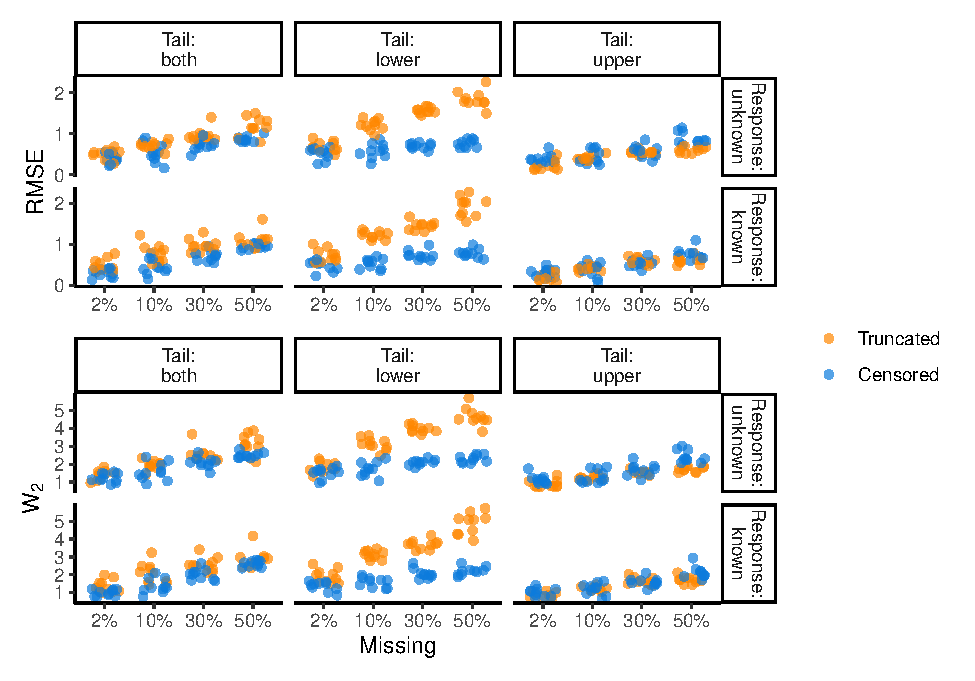
\includegraphics[keepaspectratio]{index_files/figure-pdf/fig-LBA-model-1.pdf}}

{\noindent \emph{Note.} Model root mean squared errors (RMSE) and
quadratic Wasserstein distances (\(W_2\)) for the linear ballistic
accumulator model (LBA). Lower RMSE and \(W_2\) indicate better
parameter recovery.}

\end{figure}

Figure~\ref{fig-LBA-pars} shows the \(W_2\) for each LBA parameter. In
accordance with Figure~\ref{fig-LBA-model}, lower censoring resulted in
similar or lower \(W_2\)s than lower truncation. Especially the boundary
\(B\), non-decision time \(t_0\), and mean evidence accumulation rate
\(v\) showed better parameter recovery for censoring compared to
truncation when responses are unknown, while lower censoring with
responses known improved parameter recovery for all parameters. With
both tails missing, censoring showed better parameter recovery than
truncation for most parameters, but worse recovery for starting point
variability \(A\) and mean evidence accumulation rate \(v\), explaining
the similar RMSE and \(W_2\) in Figure~\ref{fig-LBA-model}. Lastly, when
the upper tail was missing, truncation recovered the parameters
similarly to censoring, with truncation showing better parameter
recovery of starting point variability \(A\).

\phantomsection\label{cell-fig-LBA-pars}
\begin{figure}[H]

{\caption{{\(W_2\) by Parameter for the LBA}{\label{fig-LBA-pars}}}}

\pandocbounded{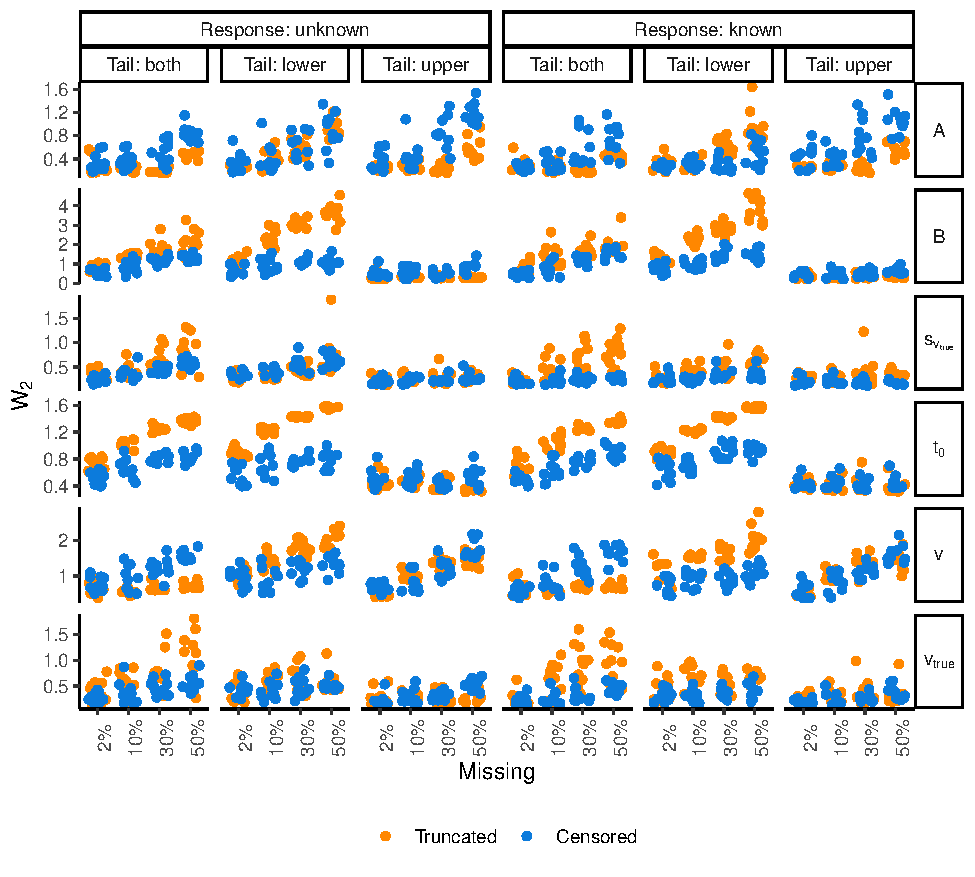
\includegraphics[keepaspectratio]{index_files/figure-pdf/fig-LBA-pars-1.pdf}}

{\noindent \emph{Note.} Quadratic Wasserstein distances (\(W_2\))
between the true LBA parameters and the LBA parameter posteriors. Each
row denotes the LBA parameter shown in the boxes on the right, and each
column denotes the tail that was missing and whether responses are known
or unknown.}

\end{figure}

\subsection{Log-Normal Race Model}\label{log-normal-race-model}

For the LNR, both upper and lower censoring showed better parameter
recovery as expected. For the lower and upper tail simulation,
Figure~\ref{fig-LNR-model} shows the expected pattern of increasing
RMSEs and \(W_2\)s for truncation while censoring RMSEs and \(W_2\)s
remain low. Unexpectedly, missing values in both tails did not result in
the same clear pattern, especially for \(W_2\). This difference between
RMSEs and \(W_2\) indicate that although the medians of censoring
posterior distributions were closer to the true parameter values, the
complete posteriors had similar distances to the true parameter values
for censoring compared to truncation.

\phantomsection\label{cell-fig-LNR-model}
\begin{figure}[H]

{\caption{{Model RMSE and \(W_2\) for the LNR}{\label{fig-LNR-model}}}}

\pandocbounded{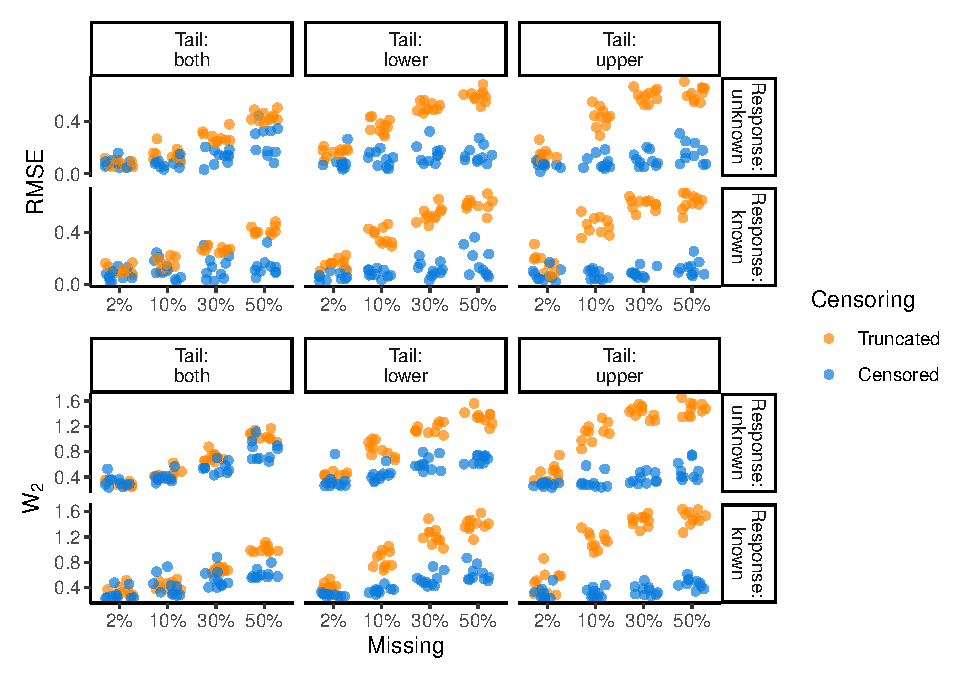
\includegraphics[keepaspectratio]{index_files/figure-pdf/fig-LNR-model-1.pdf}}

{\noindent \emph{Note.} Model root mean squared errors (RMSE) and
quadratic Wasserstein distances (\(W_2\)) for the log-normal race model
(LNR). Lower RMSE and \(W_2\) indicate better parameter recovery.}

\end{figure}

Looking at the parameter \(W_2\)s in Figure~\ref{fig-LNR-pars}, we see
that lower truncation particularly deteriorated the estimates for the
log-normal \(\mu\) estimates \(m\) and \(m_{true}\), and non-decision
time \(t_0\) compared to lower censoring, whereas upper truncation
deteriorated the estimates for log-normal \(\sigma\) estimate \(s\) and
\(t_0\) compared to upper censoring. Surprisingly, \(W_2\)s for \(t_0\)
estimates were worse for upper truncation than lower truncation, even
though non-decision time is largely reflected by the minimum RT. When
responses were unknown, lower and two-tailed censoring had worse
parameter recovery for \(s_{true}\) than truncation. Two-tailed
censoring recovered \(m\) and \(s\) better than two-tailed truncation,
but resulted in recoveries that were similar to truncation for the other
parameters.

\phantomsection\label{cell-fig-LNR-pars}
\begin{figure}[H]

{\caption{{\(W_2\) by Parameter for the LNR}{\label{fig-LNR-pars}}}}

\pandocbounded{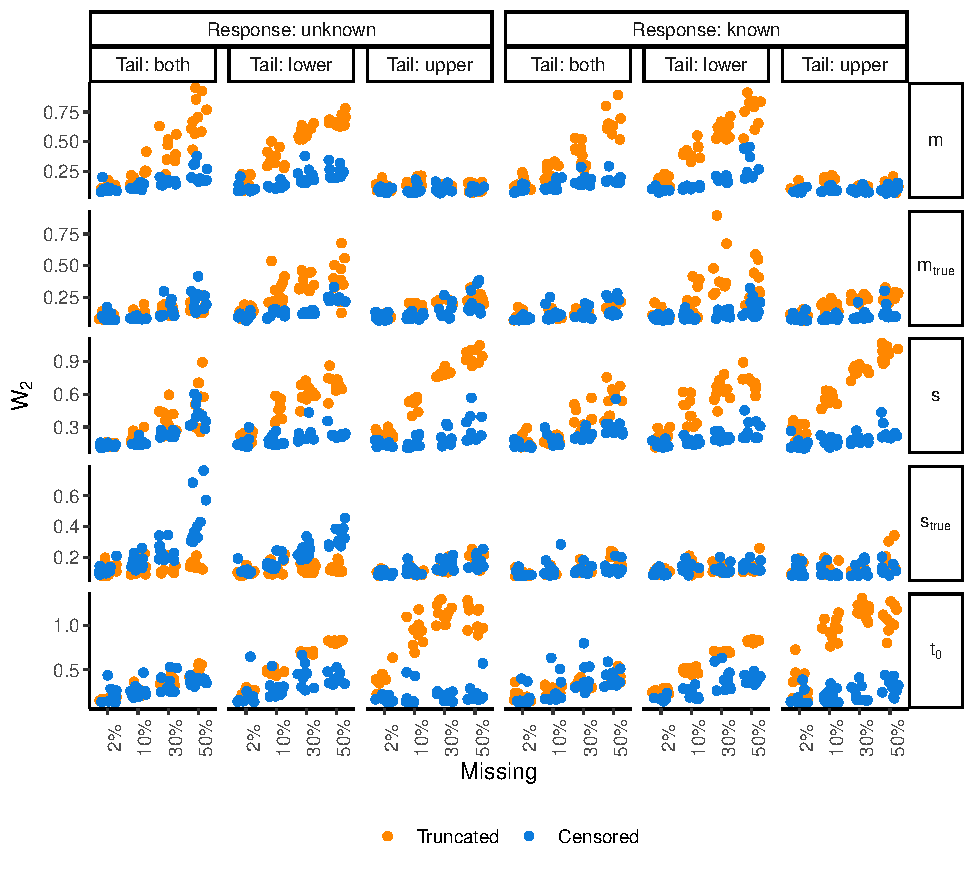
\includegraphics[keepaspectratio]{index_files/figure-pdf/fig-LNR-pars-1.pdf}}

{\noindent \emph{Note.} Quadratic Wasserstein distances (\(W_2\))
between the true Log-Normal Race (LNR) parameters and the LNR parameter
posteriors. Each row denotes the LNR parameter shown in the boxes on the
right, and each column denotes the tail that was missing and whether
responses are known or unknown.}

\end{figure}

\subsection{Racing Diffusion Model}\label{racing-diffusion-model}

Like the LBA, Figure~\ref{fig-RDM-model} shows higher RMSEs and \(W_2\)s
for lower truncation compared to lower censoring, while upper and
two-tailed censoring show similar, lower RMSEs and \(W_2\)s compared to
truncation. Only when responses were known, upper tail censoring
resulted in lower RMSE and \(W_2\) than truncation, but without a clear
separation.

\phantomsection\label{cell-fig-RDM-model}
\begin{figure}[H]

{\caption{{Model RMSE and \(W_2\) for the LNR}{\label{fig-RDM-model}}}}

\pandocbounded{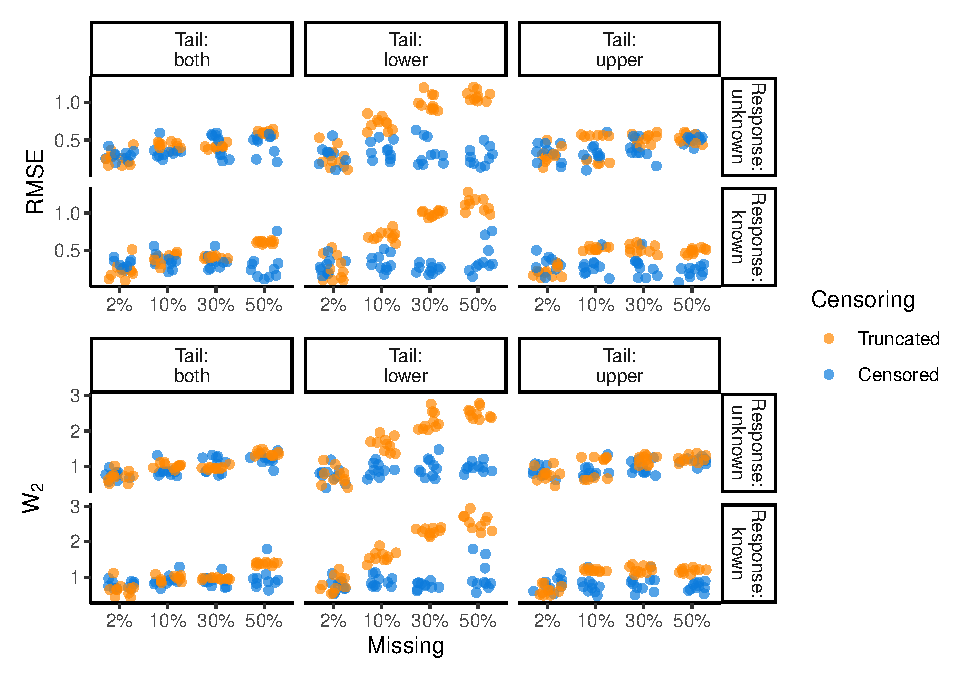
\includegraphics[keepaspectratio]{index_files/figure-pdf/fig-RDM-model-1.pdf}}

{\noindent \emph{Note.} Model root mean squared errors (RMSE) and
quadratic Wasserstein distances (\(W_2\)) for the log-normal race model
(LNR). Lower RMSE and \(W_2\) indicate better parameter recovery.}

\end{figure}

The parameter \(W_2\)s shown in Figure~\ref{fig-RDM-pars} also showed a
similar pattern to the LBA. Lower tail truncation mainly affected the
boundary parameter \(B\), the non-decision time \(t_0\), and the drift
rates \(v\) and \(v_{true}\) compared to lower censoring. The \(W^2\)s
for the drift rate of the incorrect option, \(v\), was increasing for
truncation compared to censoring, regardless of the tail or whether
responses were known. For the other parameters, upper tail and
two-tailed censoring was not particularly better or worse than
truncation, with an exception of the recovery of \(B\) and \(v_{true}\)
for upper tail censoring with responses known.

\phantomsection\label{cell-fig-RDM-pars}
\begin{figure}[H]

{\caption{{\(W_2\) by Parameter for the RDM}{\label{fig-RDM-pars}}}}

\pandocbounded{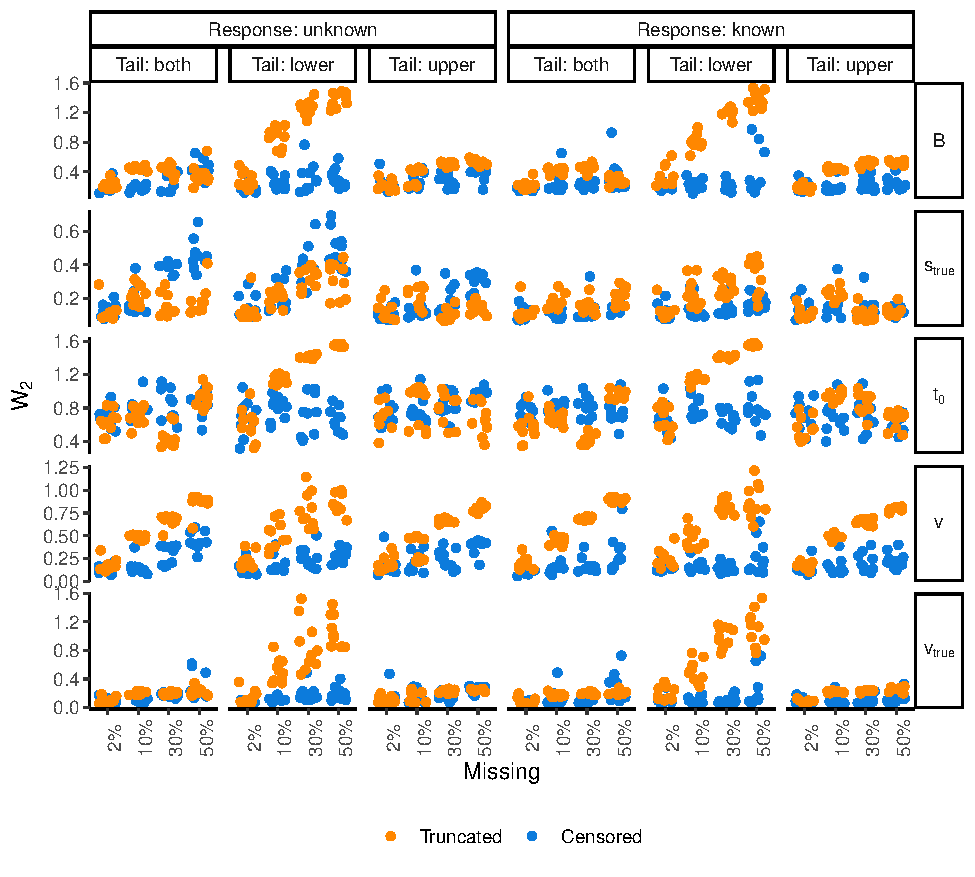
\includegraphics[keepaspectratio]{index_files/figure-pdf/fig-RDM-pars-1.pdf}}

{\noindent \emph{Note.} Quadratic Wasserstein distances (\(W_2\))
between the true racing diffusion model (RDM) parameters and the RDM
parameter posteriors. Each row denotes the RDM parameter shown in the
boxes on the right, and each column denotes the tail that was missing
and whether responses are known or unknown.}

\end{figure}

\section{Discussion}\label{discussion}

We compared censoring and truncation for three different race models:
the linear ballistic accumulator model, the log-normal race model, and
the racing diffusion model. To this end, we simulated data using
pre-specified parameter values, with missing data cutoffs based on
quantiles. The first simulation study compared asymptotic parameter
recovery upper censoring and truncation with responses known. The second
simulation used several smaller datasets for each condition in a
factorial design. It compared lower, upper and two-tailed censoring or
truncation, with either results known or unknown.

In the first simulation, parameters were recovered well for censoring,
while parameters estimated with truncation were considerably off, even
at lower percentages of missingness. Only for the RDM, 2.5\% truncation
was on par with censoring. The RDM had worse parameter recovery than the
other two models in general, with credible intervals for some parameters
missing the true parameter for each level of censoring or truncation.
Censoring still outperformed truncation in the RDM for higher
percentages of missing RTs.

The second simulation showed that the previous results did not hold with
smaller sample sizes for the LBA and RDM. However, lower truncation did
result in worse parameter recovery than censoring. For the LNR, upper
and lower truncation both resulted in better recovery than truncation,
but two-tailed truncation was closer to censoring in terms of parameter
recovery.

The results indicate that censoring improves parameter recovery
asymptotically, but in smaller numbers of trials, differences between
censoring and truncation can become inconsequential compared to random
sampling error.

Since parameter recovery for censoring was not worse than for
truncation, censoring should be preferred if parameter recovery is the
only consideration. When computation time and resources are relevant
factors, however, censoring might not always be worth the cost. When
responses were unknown, resulting in a higher number of numerical
integrals for each likelihood calculation, the PMwG sampler took more
than 28 hours in an extreme case in the second simulation. In less
extreme cases with responses known, this time was closer to 15 minutes.

To speed up the MCMC sampling for censoring, the likelihood function for
censoring was translated from R to Rcpp. This approximately doubled the
speed. In the Rcpp likelihood function, numerical integration was
implemented with RcppNumerical
(\citeproc{ref-RcppNumerical}{\textbf{RcppNumerical?}}), an Rcpp library
for numerical integration and optimization. Although this results in
faster likelihood estimations than with the \texttt{integrate} function
in R, the computation time is still considerable. To make censoring more
worthwhile, changing to a faster quadrature rule that does not have to
work for complicated multimodal functions might be beneficial.

The simulations in this paper all used non-hierarchical models. Since
the second simulation seems to have been more affected by random error
than by truncation, future simulations might use hierarchical modeling,
which is less affected by random error for single participants, but
instead shrinks more extreme values to group level means
(\citeproc{ref-shrinkage}{\textbf{shrinkage?}}), making the inference
more robust against random sampling error. Hierarchical models are
increasingly used and it remains unclear how censoring and truncation
affects hierarchical model estimation.

Another avenue that remains uninvestigated is how contamination ties
into censoring and truncation. Since truncation can remove outliers,
truncation could potentially lead to better parameter recovery than
censoring would in the presence of contaminant RTs. On the other hand,
MCMC methods also allow for the explicit modeling of contaminants. The
likelihood function that was implemented in EMC2 allows for combinations
of censoring, truncation, and explicit contaminant modeling, and future
simulations could investigate how combinations of these methods might
lead to better parameter recovery.

How researchers handle outliers and missing data can greatly affect the
outcomes of their research. Our results suggest that ignoring values
outside of a prespecified response window or outside of common outlier
thresholds can bias race model estimates. Although censoring can be
computationally costly, it should be the default over truncation when
the objective is accurate estimation of latent cognitive parameters.

\newpage{}

\section{References}\label{references}

\phantomsection\label{refs}
\begin{CSLReferences}{1}{0}
\bibitem[\citeproctext]{ref-LBA}
Brown, S. D., \& Heathcote, A. (2008). The simplest complete model of
choice response time: Linear ballistic accumulation. \emph{Cognitive
Psychology}, \emph{57}(3), 153--178.
\url{https://doi.org/10.1016/j.cogpsych.2007.12.002}

\bibitem[\citeproctext]{ref-MLcensoring}
Dolan, C. V., Van der Maas, H. L., \& Molenaar, P. C. (2002). A
framework for ML estimation of parameters of (mixtures of) common
reaction time distributions given optional truncation or censoring.
\emph{Behavior Research Methods, Instruments, \& Computers}, \emph{34},
304--323. \url{https://doi.org/10.3758/BF03195458}

\bibitem[\citeproctext]{ref-dualprocess}
Evans, J. St. B. T. (2003). In two minds: Dual-process accounts of
reasoning. \emph{Trends in Cognitive Sciences}, \emph{7}(10), 454--459.
\url{https://doi.org/10.1016/j.tics.2003.08.012}

\bibitem[\citeproctext]{ref-LNR}
Heathcote, A., \& Love, J. (2012). Linear deterministic accumulator
models of simple choice. \emph{Frontiers in Psychology}, \emph{3}.
\url{https://doi.org/10.3389/fpsyg.2012.00292}

\bibitem[\citeproctext]{ref-miller}
Miller, J. (2023). Outlier exclusion procedures for reaction time
analysis: The cures are generally worse than the disease. \emph{Journal
of Experimental Psychology: General}.
\url{https://doi.org/10.1037/xge0001450}

\bibitem[\citeproctext]{ref-outliersRatcliff}
Ratcliff, R. (1993). Methods for dealing with reaction time outliers.
\emph{Psychological Bulletin}, \emph{114}(3), 510.
\url{https://doi.org/10.1037/0033-2909.114.3.510}

\bibitem[\citeproctext]{ref-EMC2}
Stevenson, N., Donzallaz, M. C., Innes, R. J., Forstmann, B., Matzke,
D., \& Heathcote, P., Andrew. (2024). \emph{EMC2: An r package for
cognitive models of choice}. \url{https://doi.org/10.31234/osf.io/2e4dq}

\bibitem[\citeproctext]{ref-RDM}
Tillman, G., Van Zandt, T., \& Logan, G. D. (2020). Sequential sampling
models without random between-trial variability: The racing diffusion
model of speeded decision making. \emph{Psychonomic Bulletin \& Review},
\emph{27}(5), 911--936. \url{https://doi.org/10.3758/s13423-020-01719-6}

\bibitem[\citeproctext]{ref-ulrichmiller}
Ulrich, R., \& Miller, J. (1994). Effects of truncation on reaction time
analysis. \emph{Journal of Experimental Psychology: General},
\emph{123}(1), 34. \url{https://doi.org/10.1037//0096-3445.123.1.34}

\end{CSLReferences}

\appendix

\section{Supplementary Materials Study 1}\label{apx-study1}

\section{Supplementary Materials Study 2}\label{apx-study2}

\subsection{Linear Ballistic Accumulator
Model}\label{linear-ballistic-accumulator-model-1}

\subsubsection{Model Distances}\label{model-distances}

\phantomsection\label{cell-fig-MAE-both-LBA}
\begin{figure}

{\caption{{Mean Absolute Errors for the Linear Ballistic Accumulator
(LBA)}{\label{fig-MAE-both-LBA}}}}

\pandocbounded{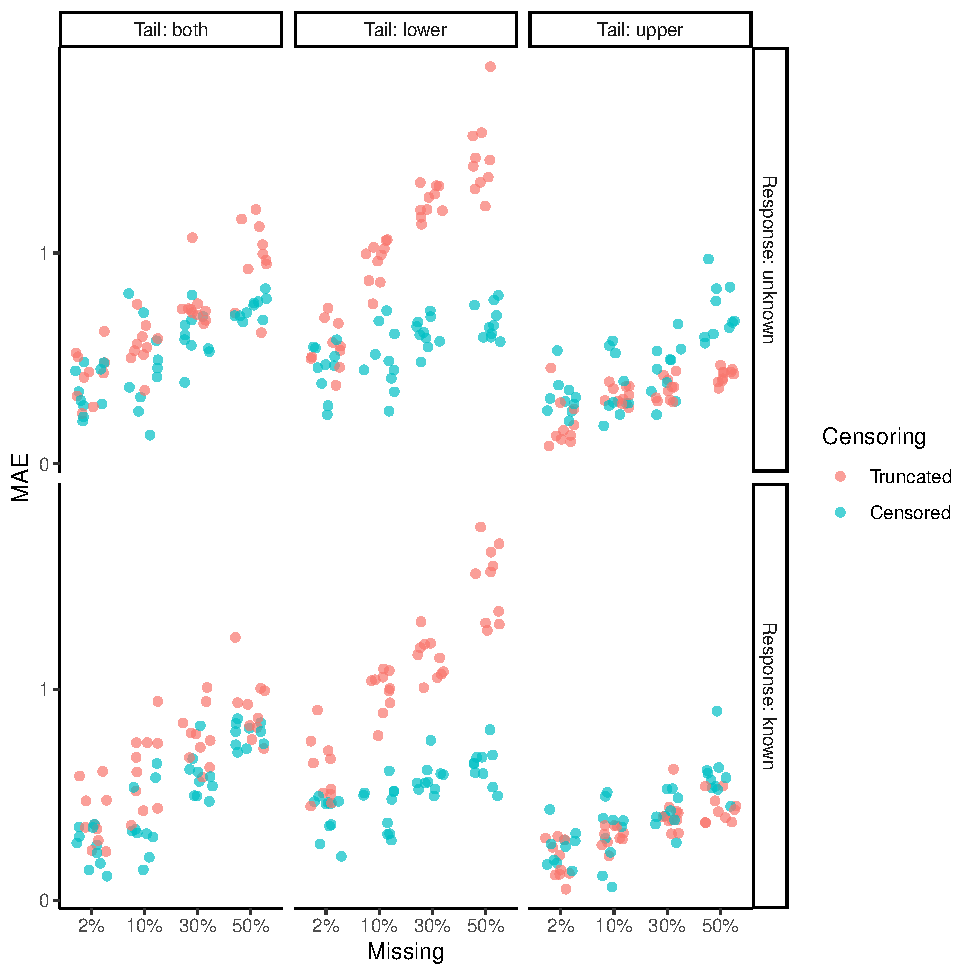
\includegraphics[keepaspectratio]{index_files/figure-pdf/fig-MAE-both-LBA-1.pdf}}

{\noindent \emph{Note.} }

\end{figure}

\phantomsection\label{cell-fig-R-both-LBA}
\begin{figure}

{\caption{{R for the linear ballistic accumulator
(LBA)}{\label{fig-R-both-LBA}}}}

\pandocbounded{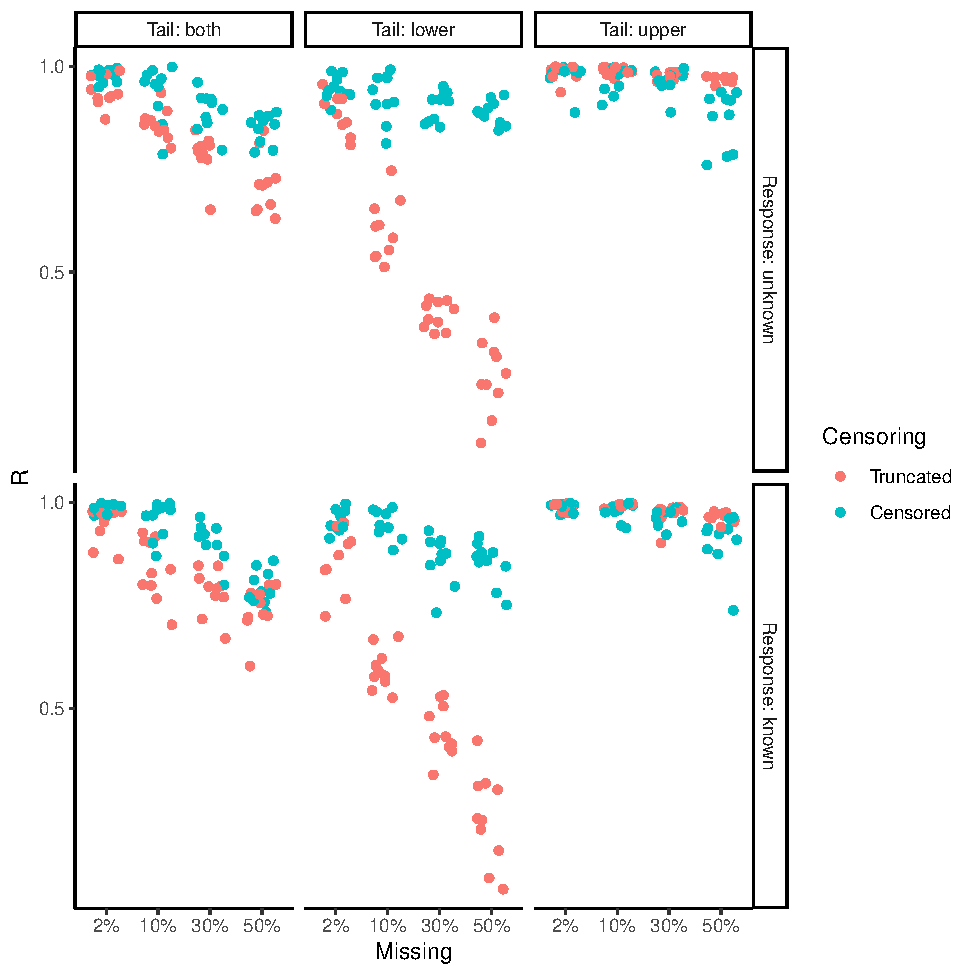
\includegraphics[keepaspectratio]{index_files/figure-pdf/fig-R-both-LBA-1.pdf}}

{\noindent \emph{Note.} Something something}

\end{figure}

\subsubsection{Credible Intervals}\label{credible-intervals}

\paragraph{Upper Tail.}\label{upper-tail}

\phantomsection\label{cell-fig-LBA-upper-known}
\begin{figure}[H]

\caption{\label{fig-LBA-upper-known}Linear Ballistic Accumulator
Posterior Medians and 95\% Credible Intervals with Missing Upper Tail
and Responses Known}

\centering{

\pandocbounded{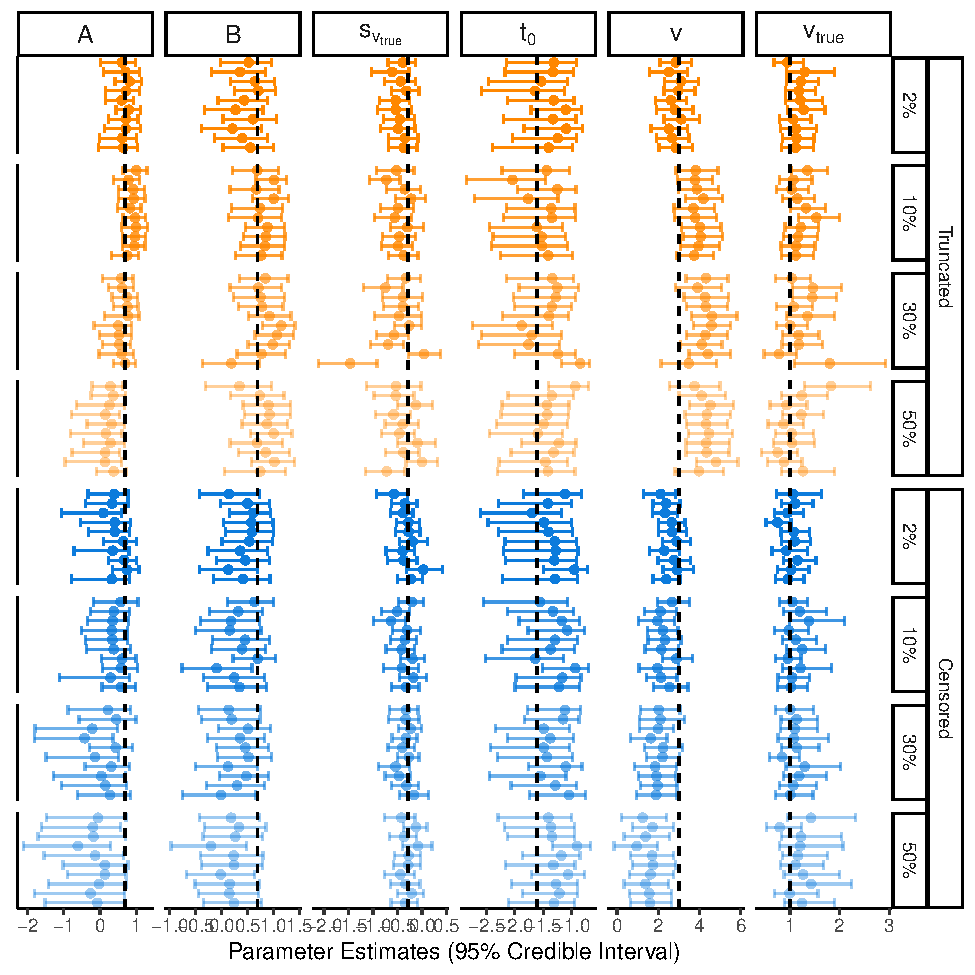
\includegraphics[keepaspectratio]{index_files/figure-pdf/fig-LBA-upper-known-1.pdf}}

}

\end{figure}%

\phantomsection\label{cell-fig-LBA-upper-unknown}
\begin{figure}[H]

\caption{\label{fig-LBA-upper-unknown}Linear Ballistic Accumulator
Posterior Medians and 95\% Credible Intervals with Missing Upper Tail
and Responses Unknown}

\centering{

\pandocbounded{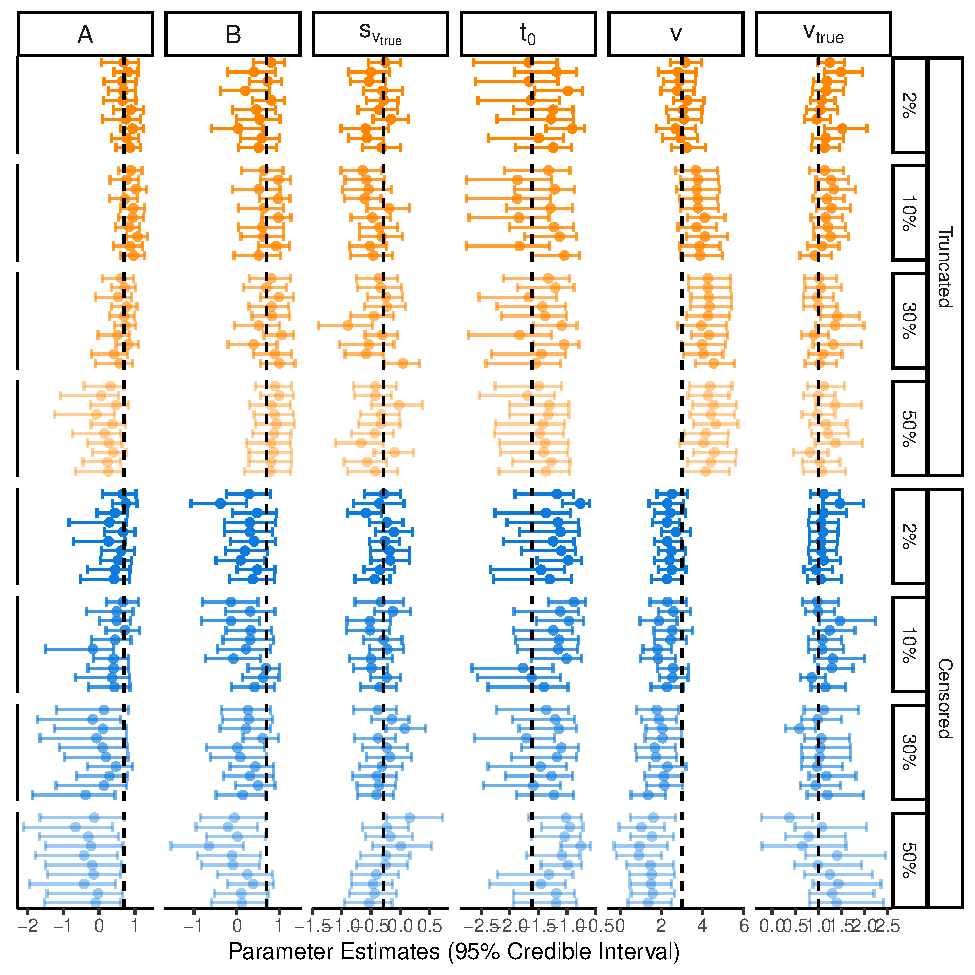
\includegraphics[keepaspectratio]{index_files/figure-pdf/fig-LBA-upper-unknown-1.pdf}}

}

\end{figure}%

\paragraph{Lower Tail.}\label{lower-tail}

\phantomsection\label{cell-fig-LBA-lower-known}
\begin{figure}[H]

\caption{\label{fig-LBA-lower-known}Linear Ballistic Accumulator
Posterior Medians and 95\% Credible Intervals with Missing Lower Tail
and Responses Known}

\centering{

\pandocbounded{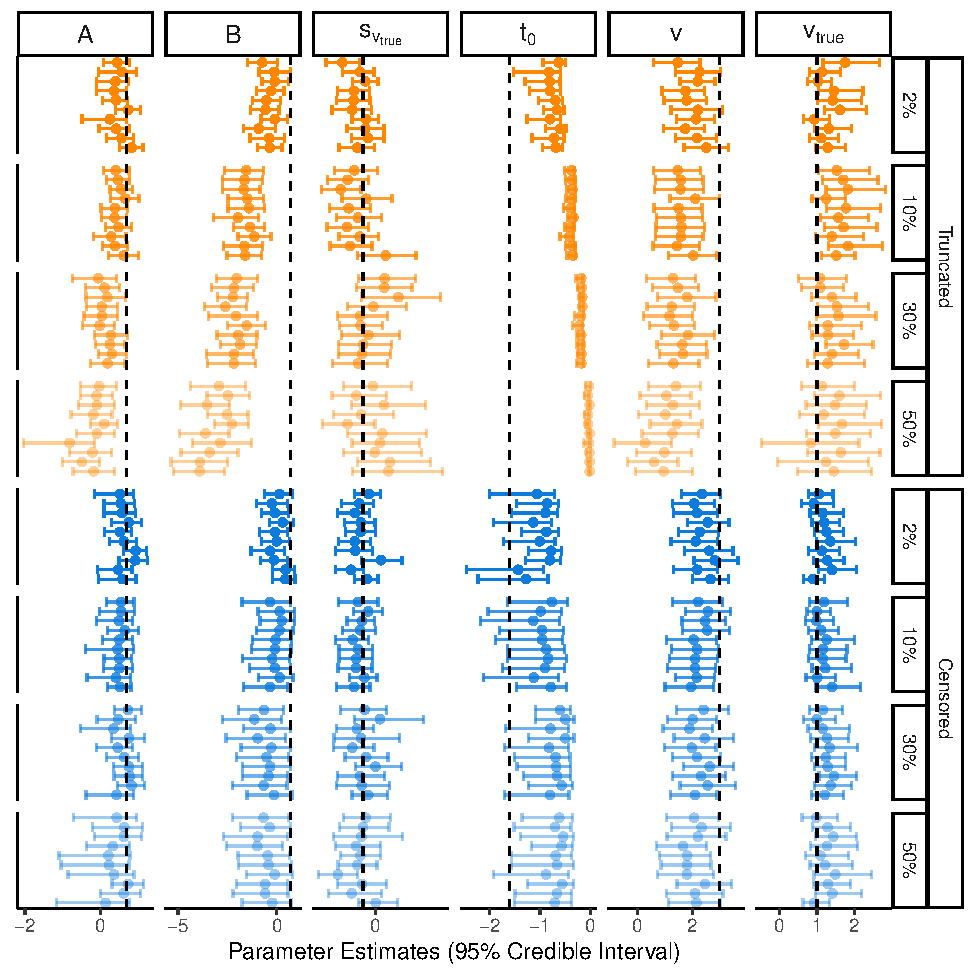
\includegraphics[keepaspectratio]{index_files/figure-pdf/fig-LBA-lower-known-1.pdf}}

}

\end{figure}%

\phantomsection\label{cell-fig-LBA-lower-unknown}
\begin{figure}[H]

\caption{\label{fig-LBA-lower-unknown}Linear Ballistic Accumulator
Posterior Medians and 95\% Credible Intervals with Missing Lower Tail
and Responses Unknown}

\centering{

\pandocbounded{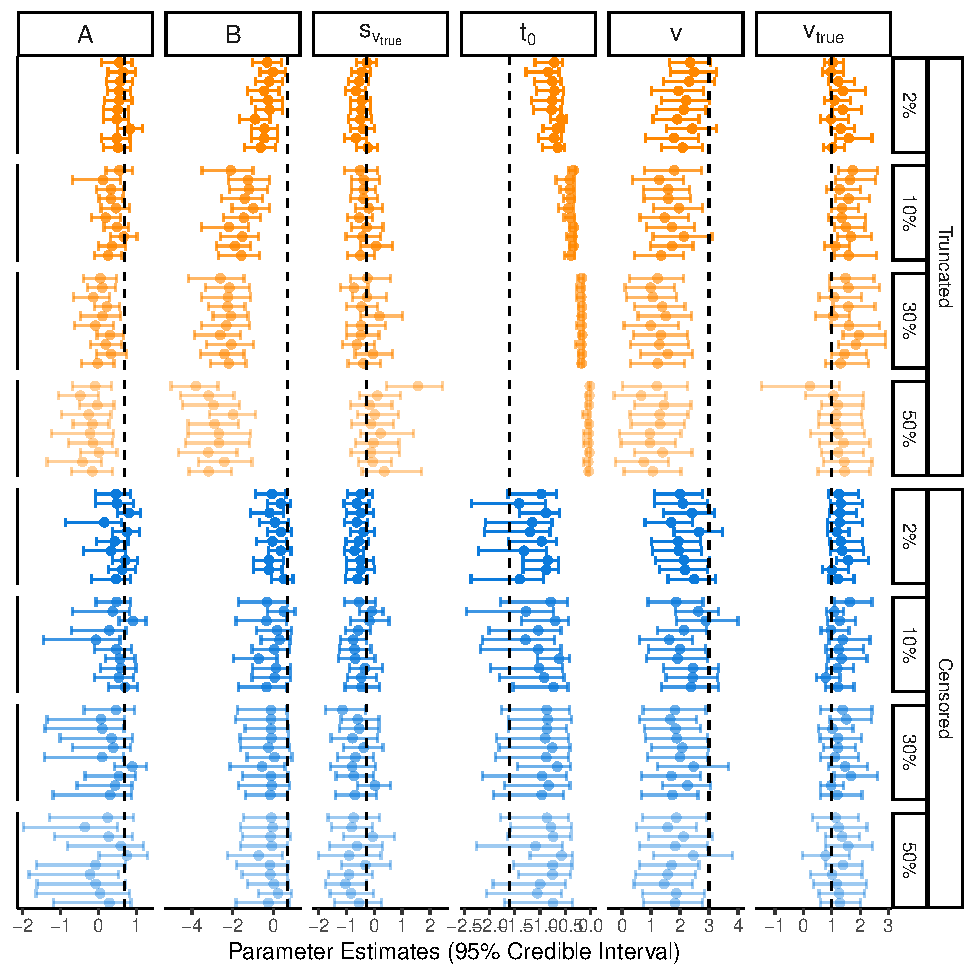
\includegraphics[keepaspectratio]{index_files/figure-pdf/fig-LBA-lower-unknown-1.pdf}}

}

\end{figure}%

\paragraph{Both Tails.}\label{both-tails}

\phantomsection\label{cell-fig-LBA-both-known}
\begin{figure}[H]

\caption{\label{fig-LBA-both-known}Linear Ballistic Accumulator
Posterior Medians and 95\% Credible Intervals with Missing Upper and
Lower Tail and Responses Known}

\centering{

\pandocbounded{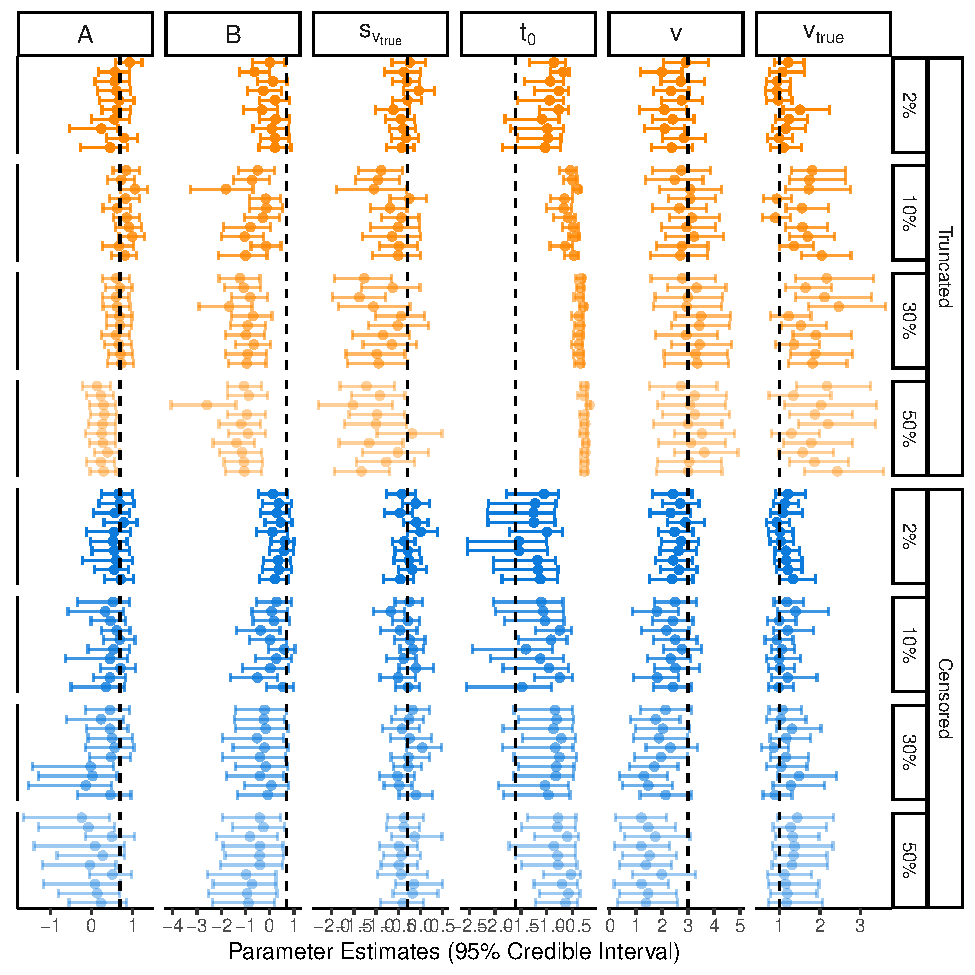
\includegraphics[keepaspectratio]{index_files/figure-pdf/fig-LBA-both-known-1.pdf}}

}

\end{figure}%

\phantomsection\label{cell-fig-LBA-both-unknown}
\begin{figure}[H]

\caption{\label{fig-LBA-both-unknown}Linear Ballistic Accumulator
Posterior Medians and 95\% Credible Intervals with Missing Upper and
Lower Tail and Responses Unknown}

\centering{

\pandocbounded{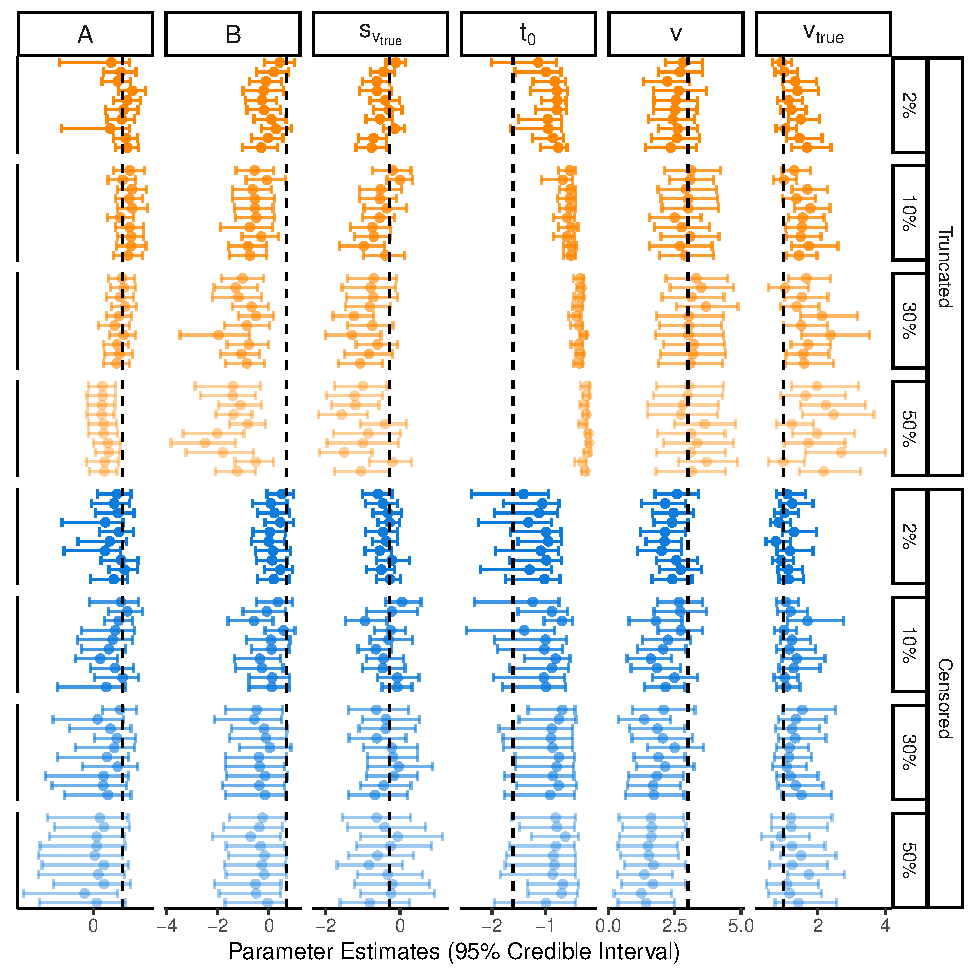
\includegraphics[keepaspectratio]{index_files/figure-pdf/fig-LBA-both-unknown-1.pdf}}

}

\end{figure}%

\subsection{Log-Normal Race Model}\label{log-normal-race-model-1}

\subsubsection{Model Distances}\label{model-distances-1}

\phantomsection\label{cell-fig-MAE-both-LNR}
\begin{figure}

{\caption{{MAE for the Log-Normal Race
(LNR)}{\label{fig-MAE-both-LNR}}}}

\pandocbounded{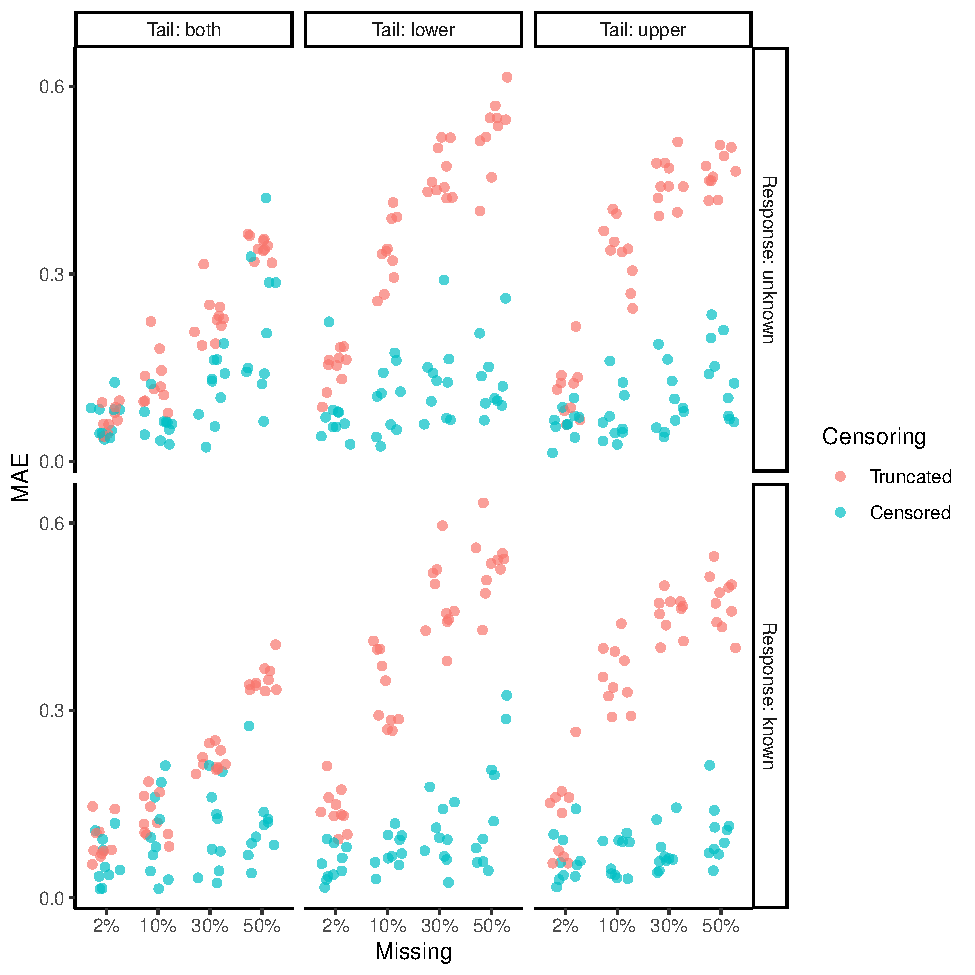
\includegraphics[keepaspectratio]{index_files/figure-pdf/fig-MAE-both-LNR-1.pdf}}

{\noindent \emph{Note.} Something something}

\end{figure}

\phantomsection\label{cell-fig-R-both-LNR}
\begin{figure}

{\caption{{R for the Log-Normal Race Model
(LNR)}{\label{fig-R-both-LNR}}}}

\pandocbounded{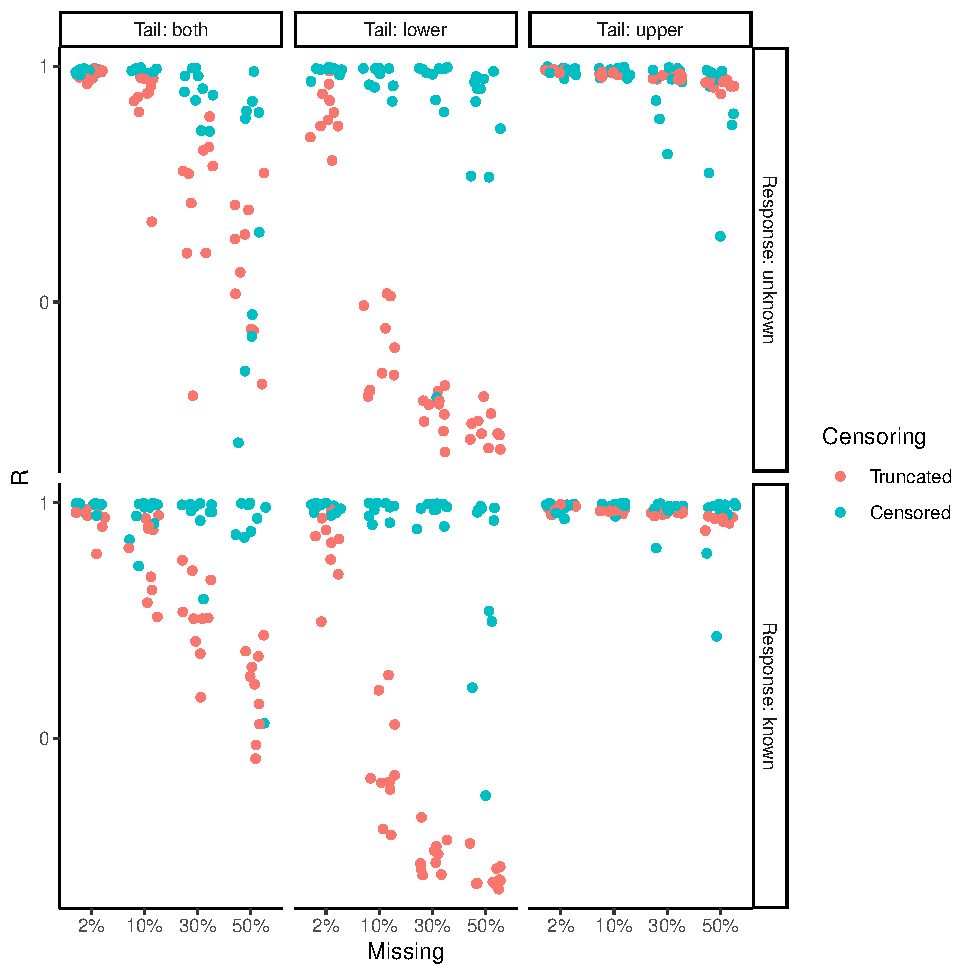
\includegraphics[keepaspectratio]{index_files/figure-pdf/fig-R-both-LNR-1.pdf}}

{\noindent \emph{Note.} Something something}

\end{figure}

\subsubsection{Credible Intervals}\label{credible-intervals-1}

\paragraph{Upper Tail.}\label{upper-tail-1}

\phantomsection\label{cell-fig-LNR-upper-known}
\begin{figure}[H]

\caption{\label{fig-LNR-upper-known}Log-Normal Race Posterior Medians
and 95\% Credible Intervals with Missing Upper Tail and Responses Known}

\centering{

\pandocbounded{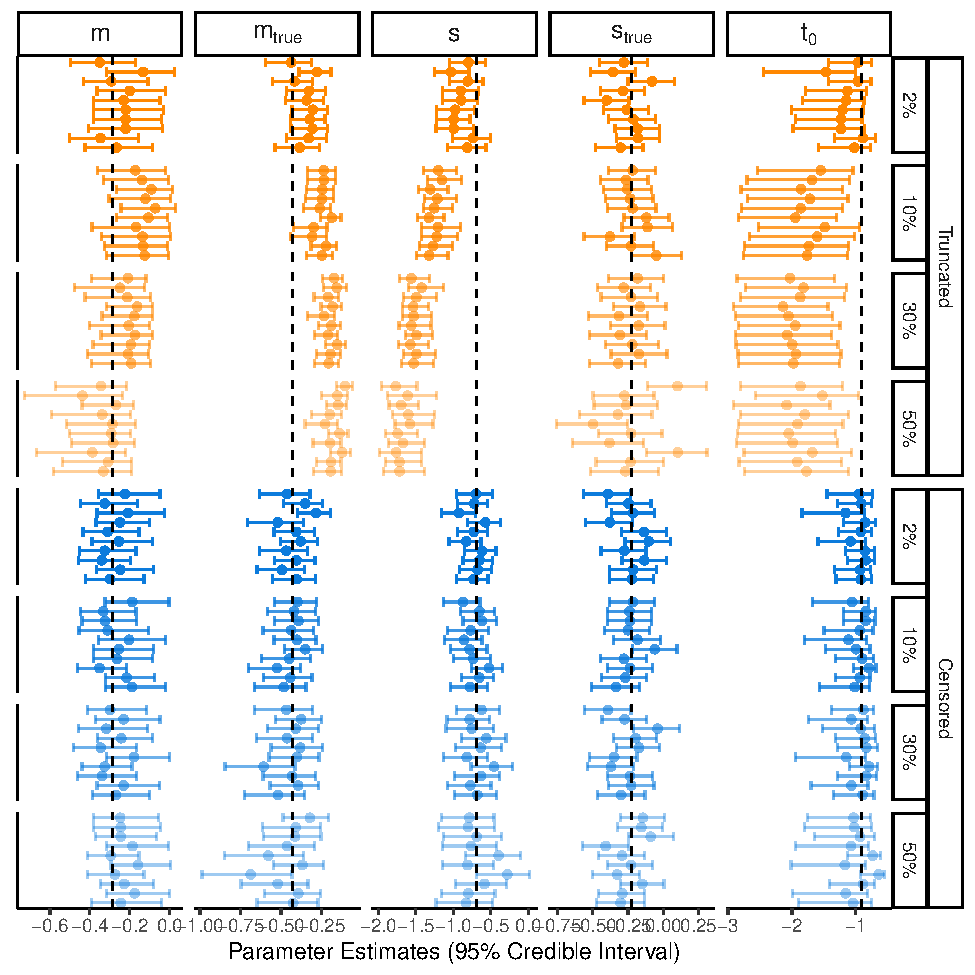
\includegraphics[keepaspectratio]{index_files/figure-pdf/fig-LNR-upper-known-1.pdf}}

}

\end{figure}%

\phantomsection\label{cell-fig-LNR-upper-unknown}
\begin{figure}[H]

\caption{\label{fig-LNR-upper-unknown}Log-Normal Race Posterior Medians
and 95\% Credible Intervals with Missing Upper Tail and Responses
Unknown}

\centering{

\pandocbounded{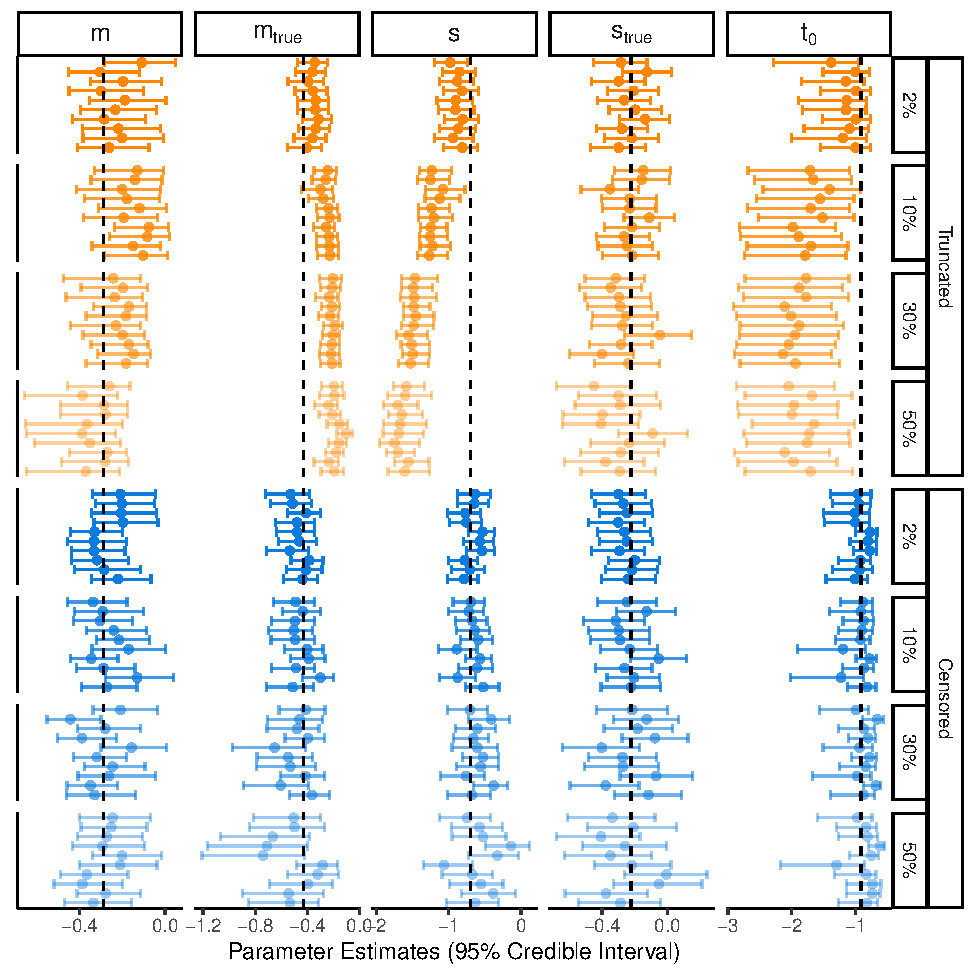
\includegraphics[keepaspectratio]{index_files/figure-pdf/fig-LNR-upper-unknown-1.pdf}}

}

\end{figure}%

\paragraph{Lower Tail.}\label{lower-tail-1}

\phantomsection\label{cell-fig-LNR-lower-known}
\begin{figure}[H]

\caption{\label{fig-LNR-lower-known}Log-Normal Race Posterior Medians
and 95\% Credible Intervals with Missing Lower Tail and Responses Known}

\centering{

\pandocbounded{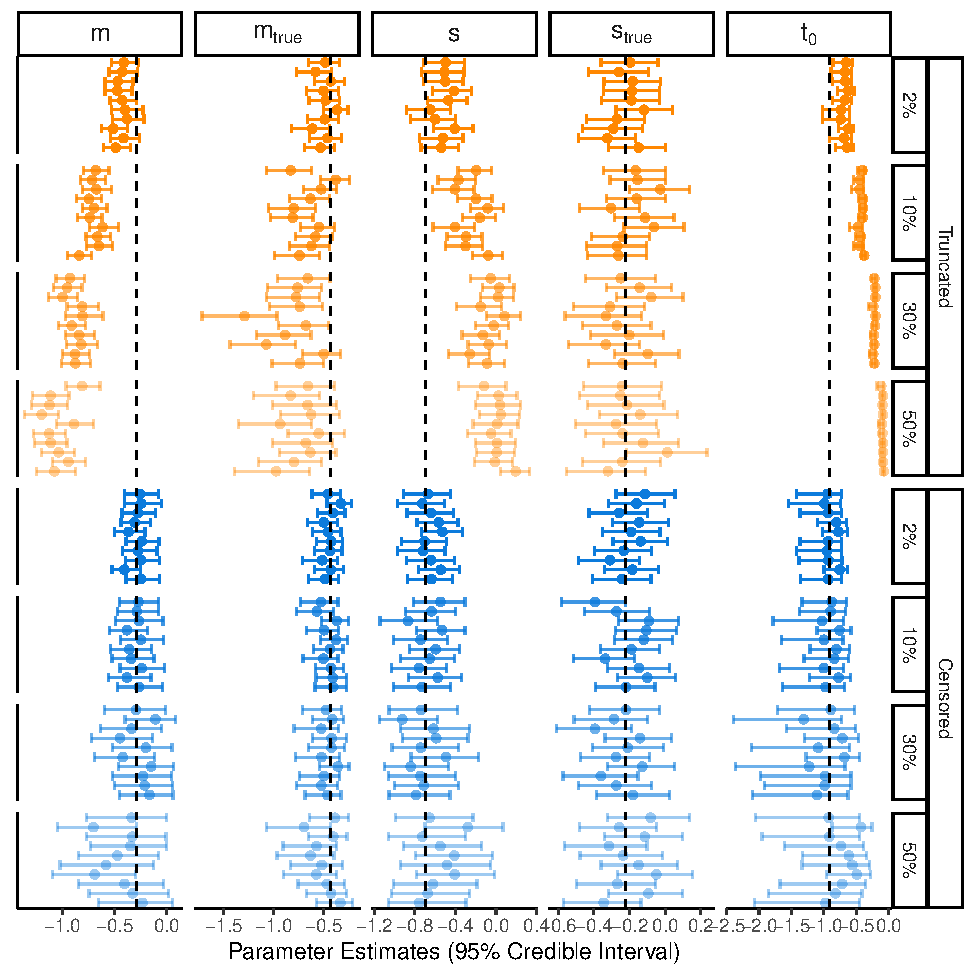
\includegraphics[keepaspectratio]{index_files/figure-pdf/fig-LNR-lower-known-1.pdf}}

}

\end{figure}%

\phantomsection\label{cell-fig-LNR-lower-unknown}
\begin{figure}[H]

\caption{\label{fig-LNR-lower-unknown}Log-Normal Race Posterior Medians
and 95\% Credible Intervals with Missing Lower Tail and Responses
Unknown}

\centering{

\pandocbounded{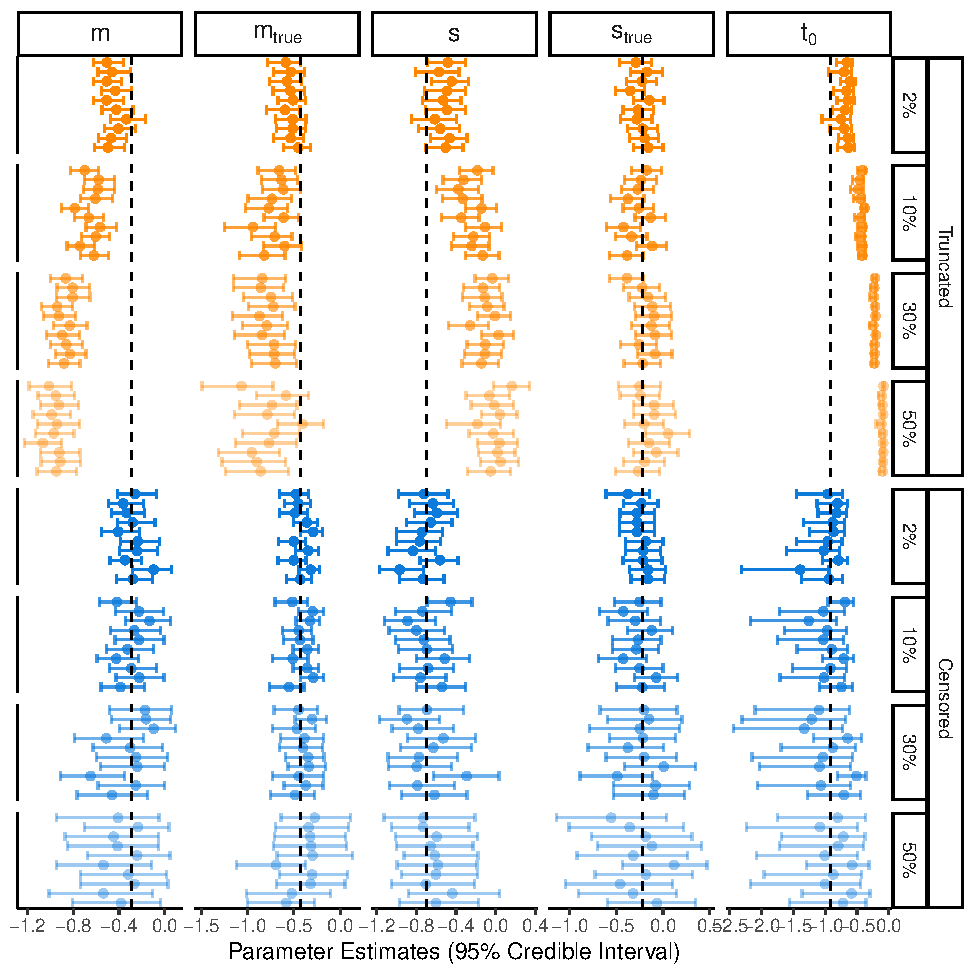
\includegraphics[keepaspectratio]{index_files/figure-pdf/fig-LNR-lower-unknown-1.pdf}}

}

\end{figure}%

\paragraph{Both Tails.}\label{both-tails-1}

\phantomsection\label{cell-fig-LNR-both-known}
\begin{figure}[H]

\caption{\label{fig-LNR-both-known}Log-Normal Race Posterior Medians and
95\% Credible Intervals with Missing Upper and Lower Tail and Responses
Known}

\centering{

\pandocbounded{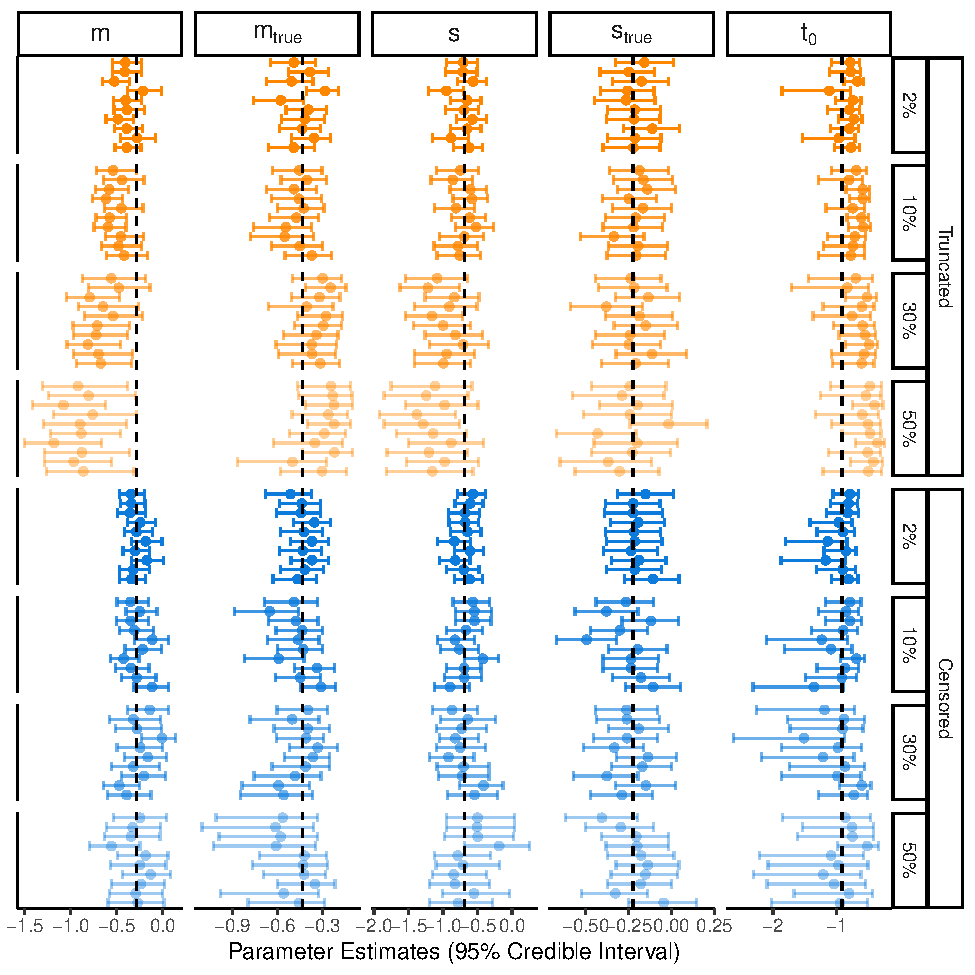
\includegraphics[keepaspectratio]{index_files/figure-pdf/fig-LNR-both-known-1.pdf}}

}

\end{figure}%

\phantomsection\label{cell-fig-LNR-both-unknown}
\begin{figure}[H]

\caption{\label{fig-LNR-both-unknown}Log-Normal Race Posterior Medians
and 95\% Credible Intervals with Missing Upper and Lower Tail and
Responses Unknown}

\centering{

\pandocbounded{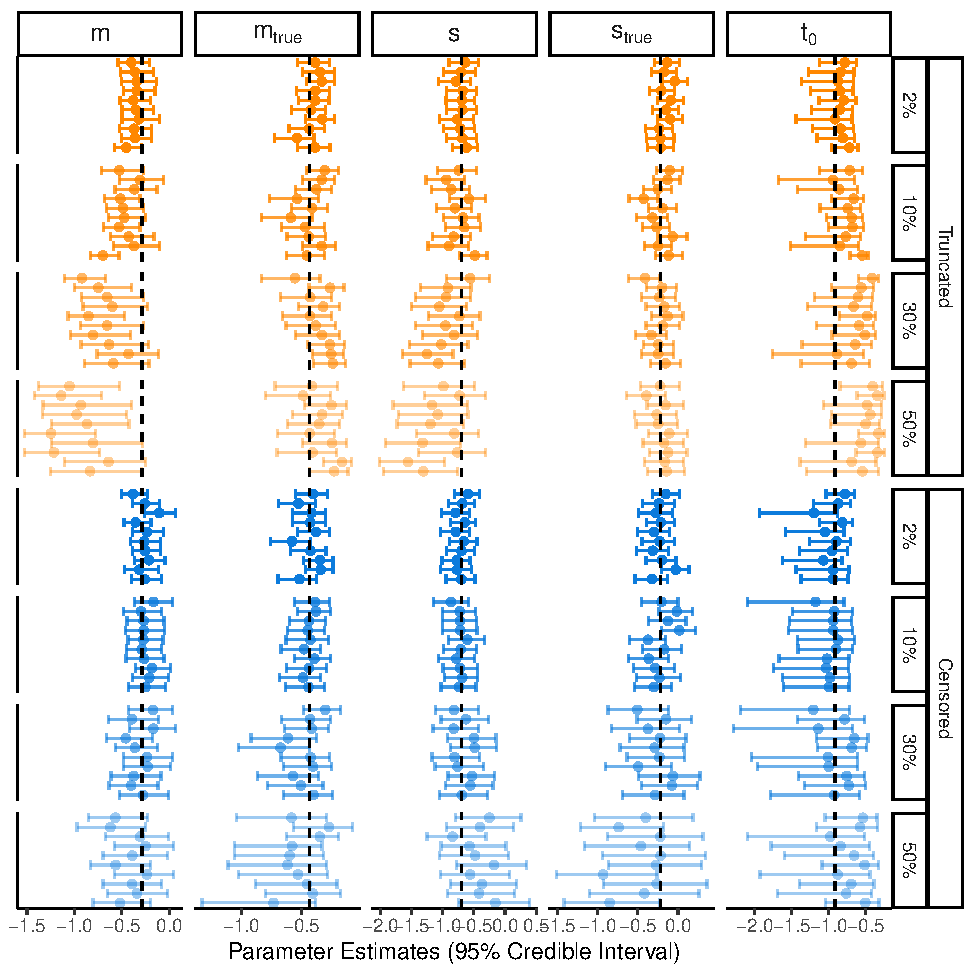
\includegraphics[keepaspectratio]{index_files/figure-pdf/fig-LNR-both-unknown-1.pdf}}

}

\end{figure}%

\subsection{Racing Diffusion Model}\label{racing-diffusion-model-1}

\subsubsection{Model Distances}\label{model-distances-2}

\phantomsection\label{cell-fig-MAE-both-RDM}
\begin{figure}

{\caption{{MAE for the Racing Diffusion Model
(RDM)}{\label{fig-MAE-both-RDM}}}}

\pandocbounded{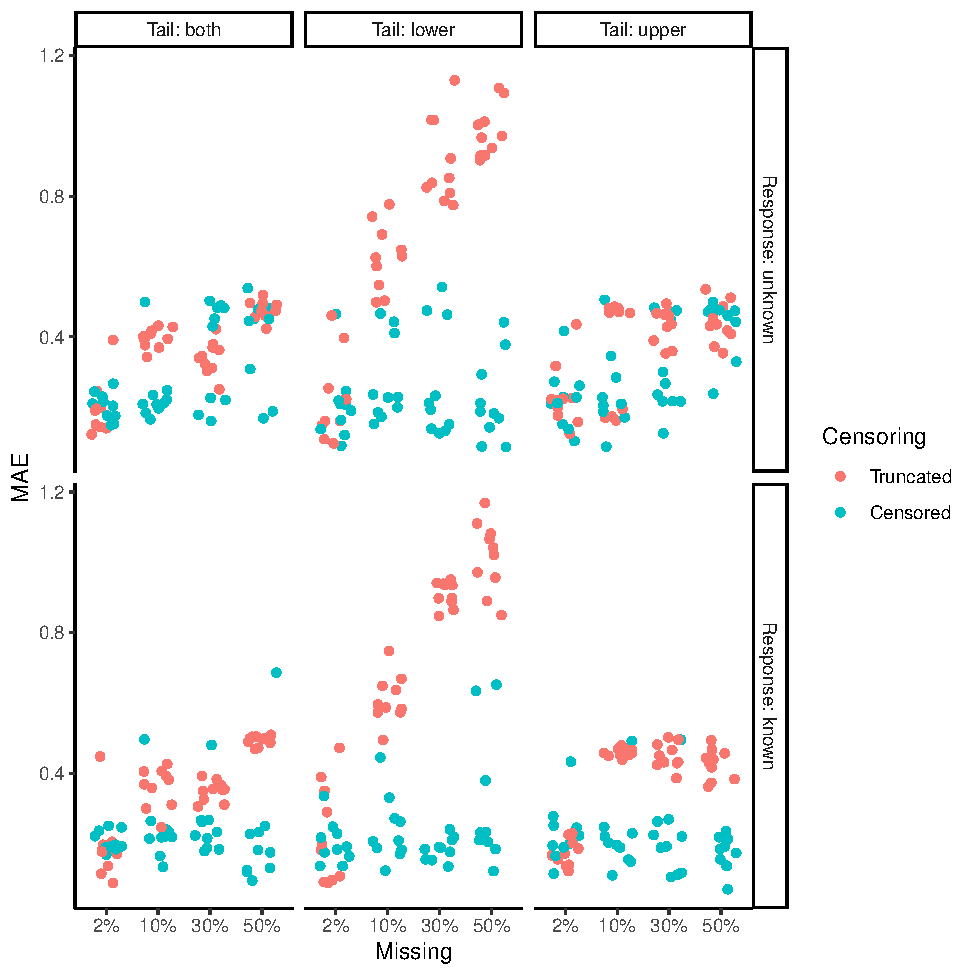
\includegraphics[keepaspectratio]{index_files/figure-pdf/fig-MAE-both-RDM-1.pdf}}

{\noindent \emph{Note.} Something something}

\end{figure}

\phantomsection\label{cell-fig-R-both-RDM}
\begin{figure}

{\caption{{R for the Racing Diffusion Model Model
(RDM)}{\label{fig-R-both-RDM}}}}

\pandocbounded{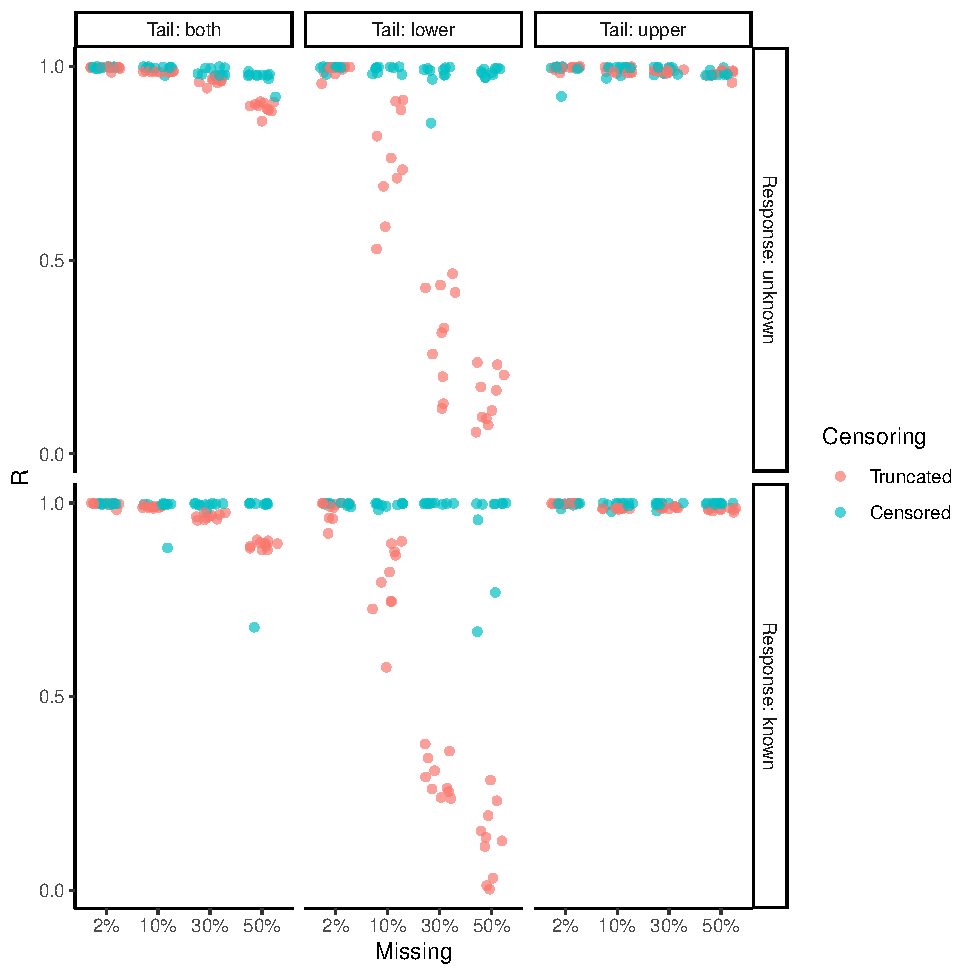
\includegraphics[keepaspectratio]{index_files/figure-pdf/fig-R-both-RDM-1.pdf}}

{\noindent \emph{Note.} Something something}

\end{figure}

\subsubsection{Credible Intervals}\label{credible-intervals-2}

\paragraph{Upper Tail.}\label{upper-tail-2}

\phantomsection\label{cell-fig-RDM-upper-known}
\begin{figure}[H]

\caption{\label{fig-RDM-upper-known}Racing Diffusion Model Posterior
Medians and 95\% Credible Intervals with Missing Upper Tail and
Responses Known}

\centering{

\pandocbounded{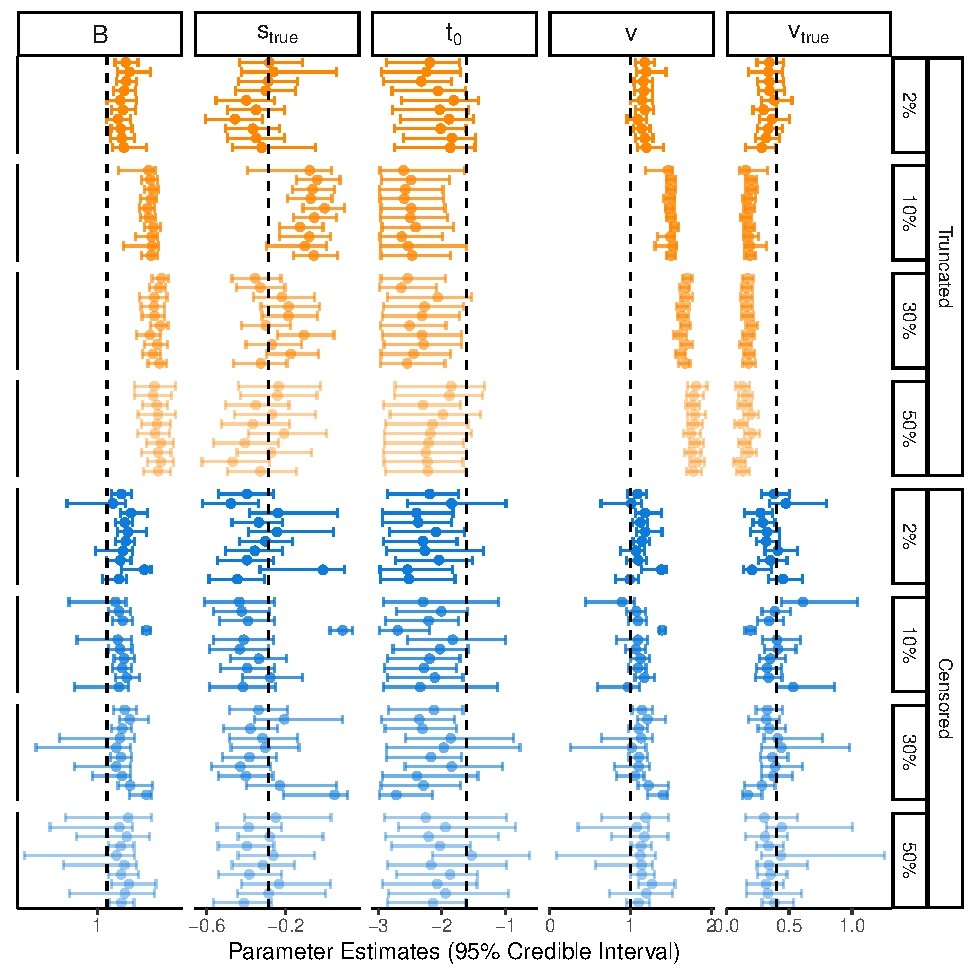
\includegraphics[keepaspectratio]{index_files/figure-pdf/fig-RDM-upper-known-1.pdf}}

}

\end{figure}%

\phantomsection\label{cell-fig-RDM-upper-unknown}
\begin{figure}[H]

\caption{\label{fig-RDM-upper-unknown}Racing Diffusion Model Posterior
Medians and 95\% Credible Intervals with Missing Upper Tail and
Responses Unknown}

\centering{

\pandocbounded{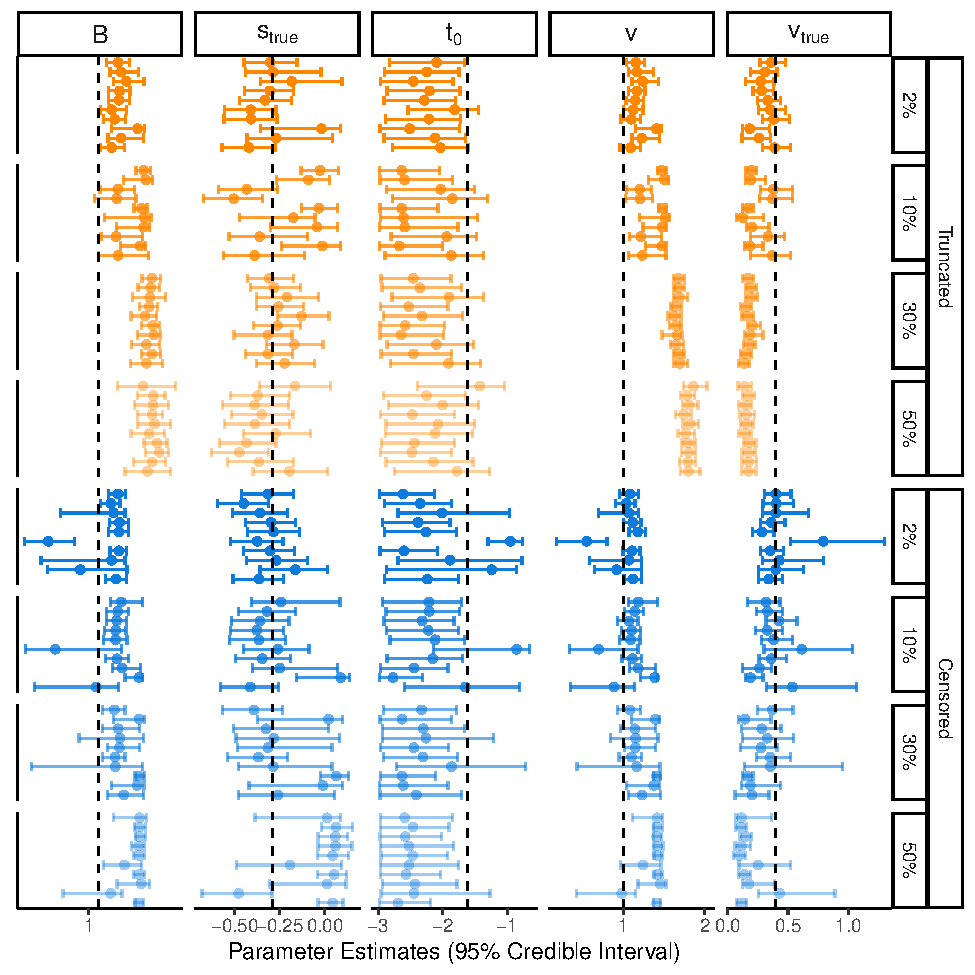
\includegraphics[keepaspectratio]{index_files/figure-pdf/fig-RDM-upper-unknown-1.pdf}}

}

\end{figure}%

\paragraph{Lower Tail.}\label{lower-tail-2}

\phantomsection\label{cell-fig-RDM-lower-known}
\begin{figure}[H]

\caption{\label{fig-RDM-lower-known}Racing Diffusion Model Posterior
Medians and 95\% Credible Intervals with Missing Lower Tail and
Responses Known}

\centering{

\pandocbounded{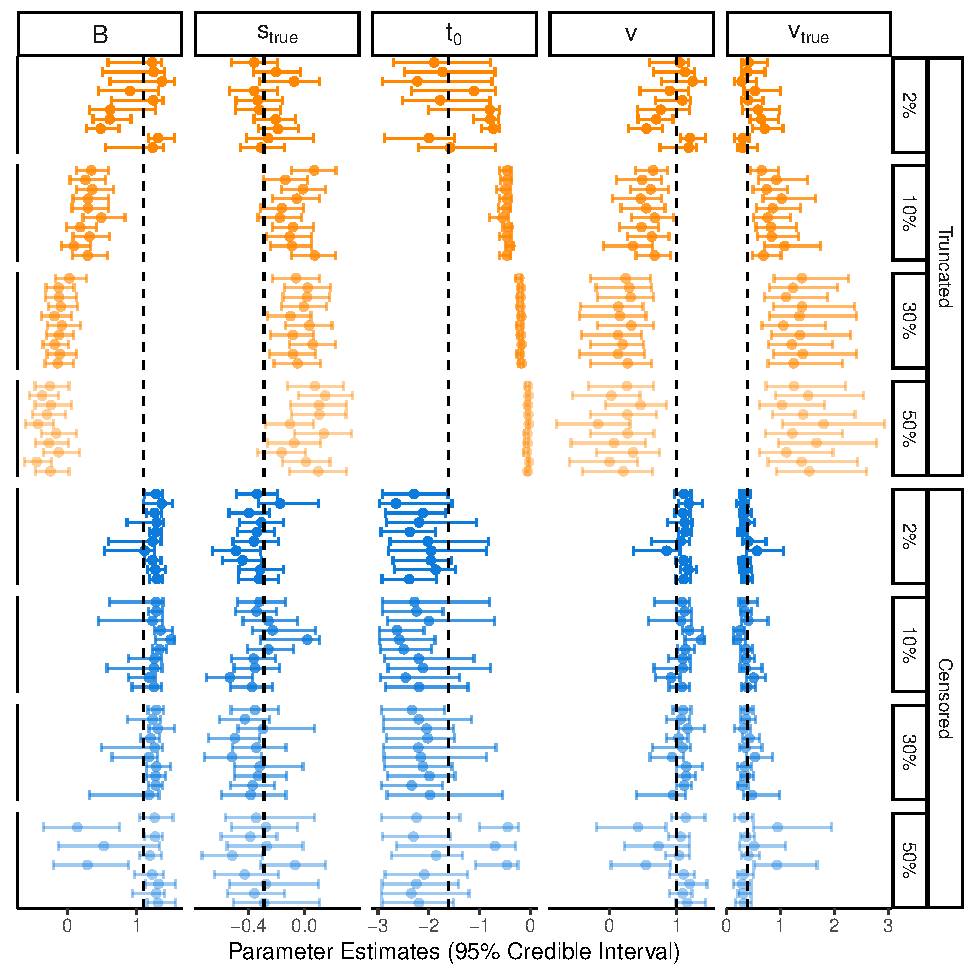
\includegraphics[keepaspectratio]{index_files/figure-pdf/fig-RDM-lower-known-1.pdf}}

}

\end{figure}%

\phantomsection\label{cell-fig-RDM-lower-unknown}
\begin{figure}[H]

\caption{\label{fig-RDM-lower-unknown}Racing Diffusion Model Posterior
Medians and 95\% Credible Intervals with Missing Lower Tail and
Responses Unknown}

\centering{

\pandocbounded{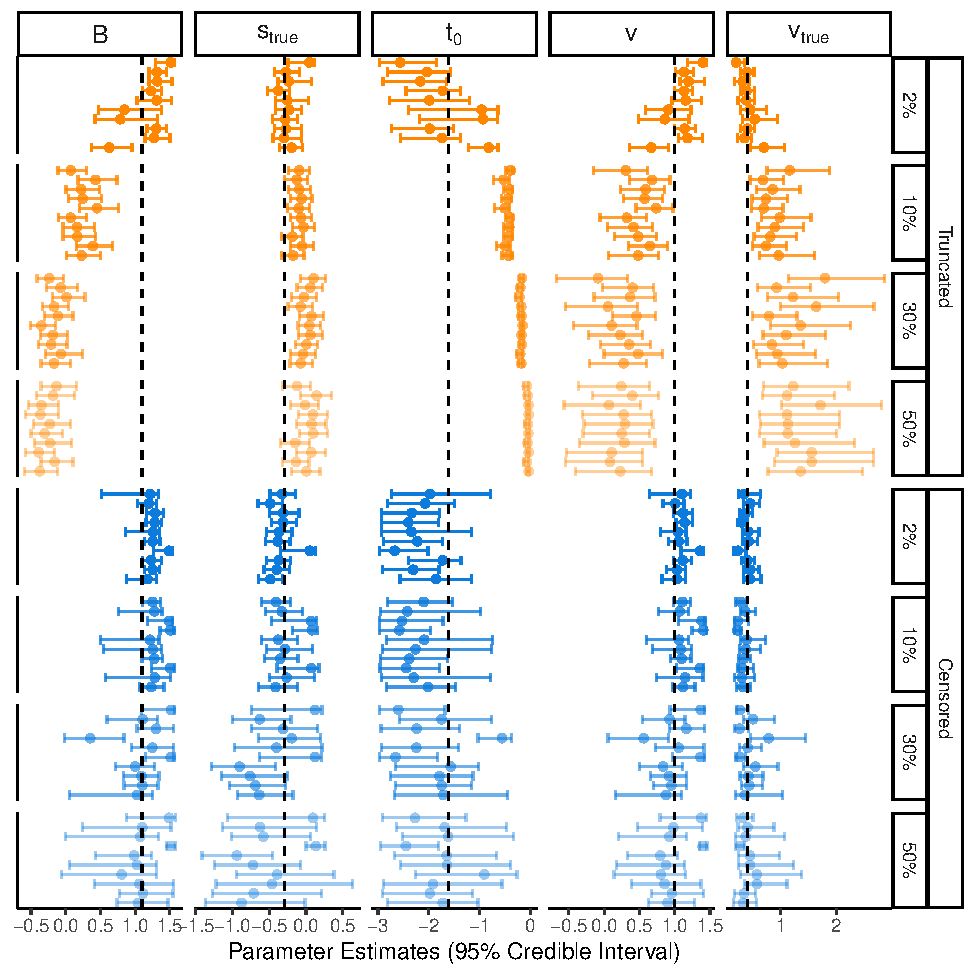
\includegraphics[keepaspectratio]{index_files/figure-pdf/fig-RDM-lower-unknown-1.pdf}}

}

\end{figure}%

\paragraph{Both Tails.}\label{both-tails-2}

\phantomsection\label{cell-fig-RDM-both-known}
\begin{figure}[H]

\caption{\label{fig-RDM-both-known}Racing Diffusion Model Posterior
Medians and 95\% Credible Intervals with Missing Upper and Lower Tail
and Responses Known}

\centering{

\pandocbounded{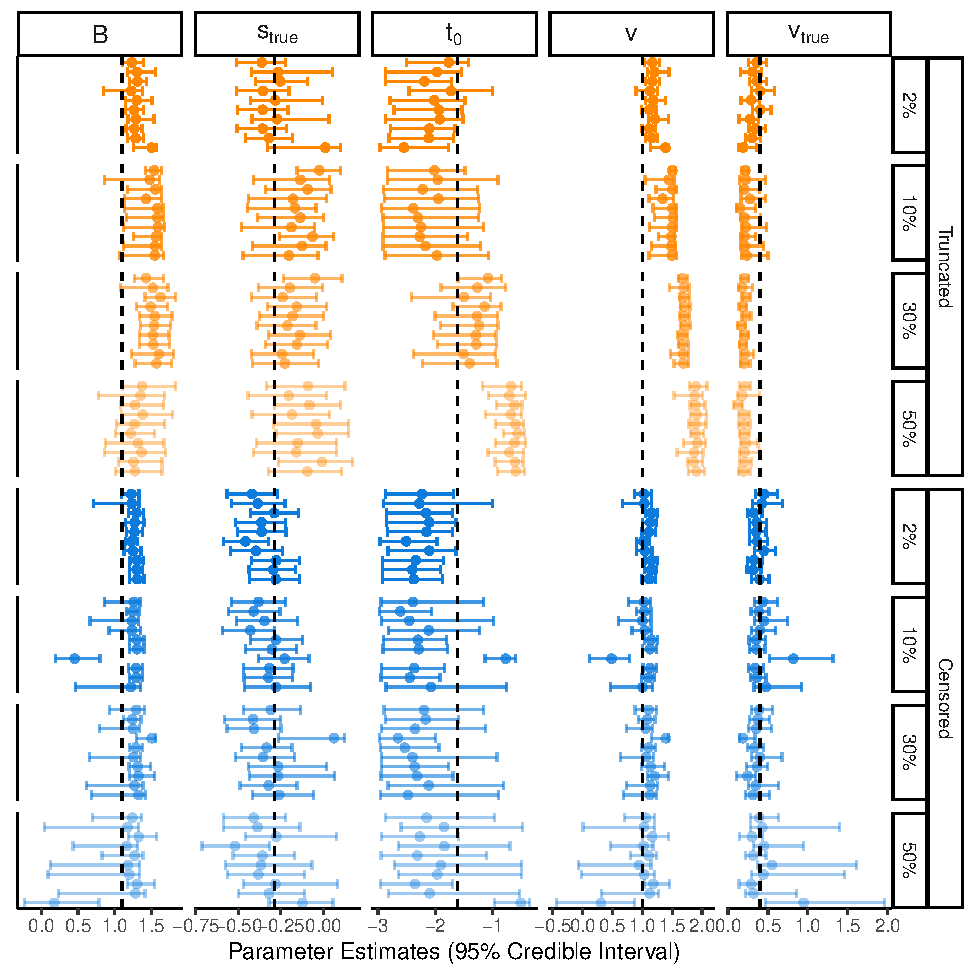
\includegraphics[keepaspectratio]{index_files/figure-pdf/fig-RDM-both-known-1.pdf}}

}

\end{figure}%

\phantomsection\label{cell-fig-RDM-both-unknown}
\begin{figure}[H]

\caption{\label{fig-RDM-both-unknown}Racing Diffusion Model Posterior
Medians and 95\% Credible Intervals with Missing Upper and Lower Tail
and Responses Unknown}

\centering{

\pandocbounded{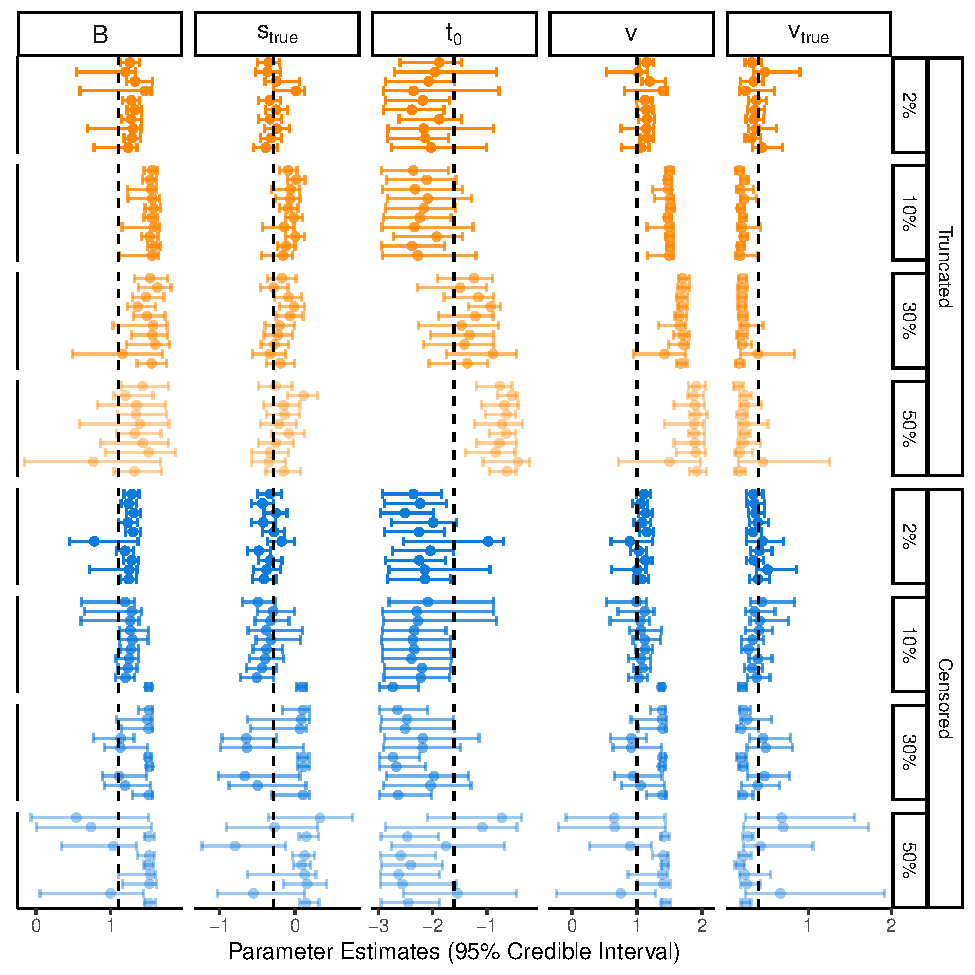
\includegraphics[keepaspectratio]{index_files/figure-pdf/fig-RDM-both-unknown-1.pdf}}

}

\end{figure}%






\end{document}
